\documentclass[a4paper,10pt]{report}

%%%%lualatex on
%\usepackage{luatextra}
\usepackage{fontspec}
%Ligatures={Contextual, Common, Historical, Rare, Discretionary}
\setmainfont[Mapping=tex-text]{Linux Libertine O}

%%%lua off
%\usepackage[utf8x]{inputenc}
%\usepackage[T1]{fontenc} 
%\usepackage{lmodern}

\usepackage{enumerate}
\usepackage{paralist}
\usepackage{graphicx}
\usepackage[french,ruled,vlined]{algorithm2e}
\usepackage[authoryear,round]{natbib}
\usepackage[frenchb]{babel}

%\usepackage[top=1.5cm,bottom=2cm,left=2.5cm,right=2.5cm]{geometry}
%\linespread{1.5}\selectfont

\usepackage{lettrine}
\usepackage{paris7}

%%Fichier Latex utilisé pour le mémoire envoyé le 26 août 2013 à Philippe Huneman et stephane schmitt frederic bouchard et nicolas bredèche.
\usepackage[colorlinks=true,urlcolor=black,citecolor=black,linkcolor=black,bookmarks=true]{hyperref}
\title{La Robotique Évolutionnaire comme modèle pour étudier la Biologie de l'Évolution }

\author{Simon Carrignon}

\begin{document}

\maketitle

\documentclass[a4paper,10pt]{report}
\usepackage{graphicx}


\begin{document}
\section*{Impact of cultural learning mechanisms on the emergence of a economi general equilibrium}

In this poster we explore a model previously build to study the interaction between cultural mechanisms and economy. In this first model groups of agents produce, consume and exchange goods. They learn and change the strategies they use to exchange goods by simply copying the more successful agents in the population.

We use for this study a variation of Approximate Bayesian Computation to explore the parameter space of the original model and to compare it to an ideal case where all exchange of goods are made under a well know economic equilibrium: the  general equilibrium (also called Walrasian equilibrium). Our method allow us to compute how likely different social learning process are able to produce a system where the emergence of a walrasian equilibrum is possible. At the same time it allow us to quantify the likelihood of the emergence of such situation under different set of fixed and limited constraints derived from historical cases studies.



\end{document}


\tableofcontents

\addcontentsline{toc}{chapter}{Introduction} 

 \chapter*{Introduction}
\section*{Algorithmique Évolutionnaire, histoire et influences}\label{sec:intro:ae}

\lettrine[lines=2]{D}{epuis} maintenant une quarantaine d'années, l'informatique assiste à l'expansion et la popularisation de toute une famille de techniques et méthodes désignées par le terme d'Algorithmique Évolutionnaire (ou AE, en anglais \emph{Evolutionnary Computation, EC})\footnote{Nous reprenons ici la traduction utilisée par \cite{schoenauer09lesalgorithmesevolutionnaires} et ne faisons pas non plus de distinction entre le terme \emph{évolutionnaire} et le terme \emph{évolutionniste}, que ce soit lorsque l'on parle d'Algorithmique Évolutionnaire ou de Robotique \'Evolutionnaire, l'un comme l'autre aurait pu être utilisé.}.
Sous cette étiquette sont regroupées des méthodes apparues plus ou moins parallèlement dans les années 60-70, dont les plus connues sont les Algorithmiques Génétiques \citep{holland75adaptationnaturalartificialsystem} et les Stratégies Évolutionnaires \citep{rechenberg73evolutionsstrategieoptimierungtechnischersystemenachprinzipienderbiologischenevolution}\footnote{Pour une brève introduction en français sur l'Algorithmique Évolutionnaire, son histoire et ses diverses sous-composantes, voir \citet{schoenauer09lesalgorithmesevolutionnaires}, pour une introduction complète et en anglais voir \citet{eiben03introductiontoevolutionarycomputing}.}.

Le point commun de ces techniques est qu'elles reprennent toutes l'idée proposée par \citet{darwin1859originspeciesbymeansnaturalselectionorpreservationfavouredracesstrugglelife} de l'évolution par sélection naturelle. L'intuition est la suivante : si la force adaptative de l'évolution telle que l'a décrite Darwin a permis l'émergence d'espèces et d'organes extrêmement adaptés aux contraintes et conditions environnementales, allant du bec du pivert parfait pour percer les arbres et attraper les insectes, à la graine couverte d'un duvet que la moindre brise transporte\footnote{Pour reprendre certains des exemples de \citet[ch. 3 notamment]{darwin1859originspeciesbymeansnaturalselectionorpreservationfavouredracesstrugglelife}.}, pourquoi la sélection naturelle ne pourrait-elle pas servir pour programmer des outils et calculer des solutions à des problèmes aussi différents que de trouver le plus court chemin entre des villes (le fameux problème du voyageur de commerce dont nous reparlerons plus tard) ou l'agencement optimal de composants électroniques sur une puce~?

\subsection*{Turing et <<\,recettes algorithmiques\,>>}
Cette intuition Turing l'avait dès 1950, dans son article que beaucoup considèrent comme fondateur de l'intelligence artificielle moderne~: <<\,Computing Machinery and Intelligence\,>>. Dans cette tentative de concevoir une machine intelligente, il propose de ne pas s'attaquer de front au <<\,développement d'un programme pour simuler l'esprit humain, mais [\ldots] plutôt d'essayer de produire l'esprit d'un enfant\,>> \citet[p. 456]{turing50computingmachineryintelligence}. L'enfant-robot produit devra avoir les mécanismes d'apprentissage capables de le faire passer correctement au stade adulte. Ainsi il n'y aurait pas besoin de programmer toutes les capacités des adultes mais simplement les méthodes d'apprentissage qui permettront aux <<\,enfants\,>> de les acquérir. Le problème est donc, selon Turing, décomposé en deux tâches : le processus d'apprentissage et la conception de la machine-enfant. Pour trouver la bonne \guillemotleft machine enfant\guillemotright, il imagine une suite d'essais/erreurs comparable, toujours selon lui, à l'évolution. Dans un premier temps une machine enfant serait conçue, à laquelle un enseignement serait dispensé. En fonction des résultats de cet enseignement <<\,il serait possible d'essayer une autre [machine-enfant] et voir si elle est mieux ou moins bien.\,>> Ainsi, par itération et accumulation de tests, de jugements de qualité et de modifications de la machine initiale, il serait possible de trouver la bonne machine capable de se développer en une <<\,machine adulte\,>> à la complexité proche de l'esprit humain.

Turing voit <<\,un lien évident entre ce processus et l'évolution\,>>. Il l'illustre par les égalités suivantes~:
\begin{quote}
   \begin{tabular}{lcl}
       Structure de la machine enfant & = &Matériel acquis par hérédité\\
       Changement dans la machine enfant&= & Mutations\\
       Sélection Naturelle &=& Jugement de l'expérimentateur\\
   \end{tabular}\\    
   \citep[p. 456]{turing50computingmachineryintelligence}
\end{quote}
Cette évolution, ajoute-t-il, <<\,l'expérimentateur, par l'exercice de son intelligence, serait capable de l'accélérer\,>>. Et voici déjà réunis tous les ingrédients que les acteurs de l'algorithmique évolutionnaire reprendront vingt ans plus tard.  

Nous reviendrons plus en détails sur la structure de la théorie de l'évolution dans le chapitre \ref{ch:evolnat} mais il est intéressant dès maintenant de noter comment cette théorie, ici résumée par Turing, peut être sujette à des entreprises <<\,d'axiomatisation\,>>. Bon nombre de biologistes à la suite de Darwin ont entrepris cette démarche et ont réfléchi à une <<\,recette idéale\,>> de l'évolution, qui résumerait les propriétés suffisantes et/ou nécessaires que doivent posséder les êtres vivants (voir pour certains à n'importe quels <<\,systèmes\,>>, vivants ou non) pour évoluer.

Cette propriété de pouvoir être résumée en courts énoncés, ainsi que le caractère formel de ces résumés (de ces recettes) fait de la théorie de l'évolution et des recettes utilisée pour la décrire, des candidates idéales pour une transcription algorithmique \citep[ch.~4, p.~48]{dennett95darwinsdangerousideaevolutionmeaningslife}. Elles apparaissent comme une suite d'instructions simples pour résoudre des problèmes complexes. Il n'est pas surprenant que, dès la naissance de l'informatique, les pères de la discipline, adeptes d'automatisation, aient pressenti le potentiel de ces recettes et aient eu envie de les reprendre à leur compte. Ils avaient à leur portée un <<\,solveur universel\,>> (en anglais \emph{universal solver}), un <<\,algorithme naturel\,>> capable de trouver automatiquement les solutions à tous ---ou au moins à une large gamme--- les problèmes possibles. Il n'y aurait plus à construire les solutions à chaque problème rencontré, mais juste à trouver un moyen d'informatiser le processus évolutif. Turing l'avait bien vu et c'est ce que les chercheurs en Algorithmique Évolutionnaire ont fait.  

Il serait tentant de conclure que Darwin, Turing et les chercheurs en Algorithmique Évolutionnaire aient tous eu la même intuition et confiance en  
\begin{quote}
   [\ldots] cette force qui adapte lentement et merveilleusement bien chaque forme aux plus complexes relations de la vie.\\
   \citep[ch. 15]{darwin1859originspeciesbymeansnaturalselectionorpreservationfavouredracesstrugglelife}
\end{quote}
Mais savoir s'ils parlent effectivement de la même <<\,force\,>>, du même processus est une question toujours débattue. Sans y répondre directement nous essayerons d'apporter quelques clefs pour y réfléchir tout au long de ce mémoire.

\subsection*{L'apport de la synthèse moderne}
Parallèlement à cette intuition turingienne quasi-visionnaire de l'applicabilité de la <<\,force darwinienne\,>> à l'informatique, qui traçait la voie à l'Algorithmique \'Evolutionnaire, l'éclosion de ces méthodes dans les années 70 s'explique mieux si elle est mise en relation avec l'histoire de la Biologie de l'époque. Nous reviendrons plus en détails sur cette histoire dans la section \ref{sec:SM}, mais pour comprendre l'avènement de l'AE, il nous paraît déjà judicieux de nous arrêter quelques instants sur cette période.

En effet, pendant les années 60 (et donc en même temps que l'apparition de l'AE), la Biologie était marquée par la fin, l'adoption et la reconnaissance de la Synthèse Moderne (SM) de la théorie de l'évolution par l'ensemble de la communauté scientifique. Cette Synthèse Moderne, appelée aussi Théorie Synthétique de l'Évolution (TSE) d'après le titre du livre de \citet{huxley1942evolution}, l'un des acteurs de l'époque, désigne une période entre les années 1930 à 1960 \footnote{Les dates exactes de la Synthèse Moderne peuvent varier suivant les auteurs et dépendent souvent de la prise en compte ou non de la phase <<\,théorique\,>>. Pour une revue critique de l'histoire de cette période voire \citep{reif00synthetictheoryevolutiongeneralproblemsgermancontributiontosynthesis}, pour une très bonne et plus large introduction à la Synthèse Moderne et à l'histoire, en français, de la pensée évolutionniste en générale voir \cite{gayon1991darwinetlapresdarwin}.} pendant laquelle un ensemble de découvertes, de modèles et de théories biologiques ont vu le jour. Cette époque a été témoin de la réconciliation des lois de Mendel (lois de transmission de caractères génétiques discrets) avec l'évolution (graduelle et continue) des êtres vivants selon Darwin et son principe de Sélection Naturelle. Cela a aussi été l'occasion d'affiner et d'agrémenter la théorie de tout un arsenal d'outils mathématiques et de modèles statistiques et conceptuels, qui n'auront qu'à être repris par les informaticiens.

Au c\oe ur de la biologie de l'évolution, là où il n'y avait que des énoncés et des hypothèses, venait désormais se greffer des équations, des chiffres et des tables statistiques, bien plus précis et simples à implémenter avec un ordinateur que des intuitions abstraites (telles celles qu'avait pu avoir Turing). Les équations de \citet{fisher1930geneticaltheorynaturalselection} pouvaient être reprises directement, les paysages adaptatifs de \cite{wrights1932rolesmutationinbreedingcrossbreedingandselectioninevolution} offraient l'outil parfait pour illustrer les espaces de recherche des solutions avec lesquels jonglent les ordinateurs \footnote{Ces paysages adaptatifs, plus souvent appelés <<\,fitness landscapes\,>> ou espaces de recherches en sciences computationnelles, se révélèrent si pertinents conceptuellement qu'ils sont devenus un élément incontournable du vocabulaire de l'Algorithmique Évolutionnaire et sont encore et toujours présentés dès l'introduction des <<\,textbooks\,>> de la discipline \citep[p. 12]{eiben03introductiontoevolutionarycomputing}} et la \emph{gene eye view} offrait les abstractions et concepts clairs et simples que pouvaient implémenter \cite{holland75adaptationnaturalartificialsystem} et les autres.


D'autres éléments de la Synthèse Moderne ont aidé à ce rapprochement et à la naissance de l'AE. Par exemple, l'introduction du langage de l'optimisation et de la théorie de l'information en biologie \citep{maynardsmith78optimizationtheoryinevolution} a permis l'application et l'échange de concepts et de procédés. Ainsi, de nouvelles méthodes d'explication ont pu être explorées\footnote{Nous reverrons plus en détails les critiques, la valeur et la portée explicative de ces modèles d'optimisation et des modèles en général, notamment à la lumière de l'approche sémantique des théories scientifiques de van Frassen comme l'a fait (entre autres) \citet{beatty1980whatswrongwithreceivedwiew} pour la biologie. Nous ne les citons ici que pour souligner le rapprochement qui s'opéra pendant le milieu du XXe siècles entre biologie et sciences computationnelles.}.

Le rapport entre cette Synthèse Moderne arrivée à maturité et l'émergence de l'Algorithmique Évolutionnaire est donc étroit. La première a offert à la seconde les outils parfaits pour que puisse être calqué le vocabulaire de la biologie sur des problèmes diverses et abstraits afin d'essayer de les résoudre en suivant une méthode, un algorithme <<\,universel\,>>. Cette superposition de concepts a rendu possible le rapprochement des vues des deux protagonistes d'une phrase de \citet[p. 179]{maynardsmith00theconceptofinformationinbiology} : <<\,[l]à où un ingénieur voit du \emph{design}, un biologiste y voit la sélection naturelle.\,>>. Pendant les années 1970, l'ingénieur a commencé à pouvoir imaginer faire du \emph{design} avec (une imitation artificielle) la Sélection Naturelle.

Néanmoins et nous essayerons de le justifier tout au long de ce mémoire, il ne faudrait pas que ce rapprochement marque trop profondément les disciplines d'Algorithmique Évolutionnaire. Si la Synthèse Moderne a été un guide et une base de départ idéale, elle ne doit pas être une entrave et les critiques qui lui sont faites doivent être étudiées et testées avec sérieux.

De plus, bien que fructueux, ce pont jeté entre problèmes informatiques et biologie de l'évolution est avant tout conceptuel et abstrait. De surcroît, il est, la majeure partie du temps, perçu comme à sens unique par les chercheurs en informatique. L'Algorithmique Évolutionnaire <<\,puise son inspiration du processus de l'évolution naturelle\,>>, annoncent \citet[p. 1]{eiben03introductiontoevolutionarycomputing} et presque tous les auteurs de la discipline. Le lien semble souvent se réduire à de simples emprunts de langage. C'est pourquoi avant d'introduire la discipline qui nous intéresse et dans laquelle l'abstraction s'estompe un peu, l'exemple classique en informatique théorique et en optimisation qu'est le problème du voyageur devrait nous aider à mieux comprendre et éclairer la nature de cette superposition linguistique entre informatique et biologie, tout en nous donnant l'occasion d'illustrer la catégorie de problèmes que peut aider à résoudre les techniques d'Algorithmique Évolutionnaire.

\section*{Le voyageur de commerce}\label{sec:intro:vc}

Dans ce problème bien connu des mathématiciens et informaticiens, un voyageur doit passer par un ensemble de villes en traversant chacune d'elles une seule fois. Le but est pour lui de parcourir le moins de kilomètres possible (d'optimiser au mieux son trajet). Comme souvent en informatique, la meilleure et plus sûre façon de trouver la solution à ce problème et de tester tous les trajets possible pour trouver le plus court parmi eux. L'inconvénient dans ce cas est que le nombre de trajets possible peut vite devenir très, très important. Ajouter une ville par laquelle notre voyageur doit passer ce n'est pas ajouter \emph{un} nouveau trajet possible mais, $M \times N$ trajets (où $M$ et $N$ sont respectivement le nombre de solutions et le nombre de villes du problème avant l'ajout de la nouvelle ville). Autrement dit : si vous aviez 6 villes à parcourir, en ajouter une seule à l'itinéraire c'est obtenir 4320 nouveaux trajets à tester. Le problème est dit NP-complet, et même des ordinateurs des milliards de fois plus puissants que le plus puissant des ordinateurs d'aujourd'hui mettraient plusieurs fois l'\^{a}ge de l'univers pour énumérer toutes les solutions possible avec une 50aine de villes.

C'est là que l'Algorithmique \'Evolutionnaire entre en jeu. Pour comprendre comment nous allons présenter sans entrer dans les détails, un algorithme génétique simple pour résoudre ce problème.

La première étape avant de lancer l'algorithme et de faire correspondre les éléments du problème aux concepts biologiques. Dans notre situation le but est de trouver le trajet le plus court, la <<\,solution\,>> du problème sera donc un trajet, autrement dit une suite de villes à traverser (par exemple Lyon, Marseille, Paris et Grenoble). Dans le monde biologique il n'y a pas de <<\,solution\,>> à proprement parler mais plutôt un <<\,résultat\,>> : des individus adaptés à leur environnement. Pour simplifier et dans la lignée des architectes de la Synthèse Moderne, l'individu est considéré comme réductible à son génome. Nous dirons ainsi que ---dans un grossière simplification qui ne veut pas rendre compte d'une réalité du monde du vivant mais simplement en extraire une heuristique utile : le résultat (les <<\,solutions\,>>) de l'évolution est un ensemble de génomes qui code pour des individus adaptés à leur environnement\footnote{Nous tenons à insister encore ici sur la valeur heuristique de cette simplification, qui, et nous le reverrons, peut poser des problèmes d'ailleurs illustrés de façon particulièrement probante en algorithmique évolutionnaire, cf \citet{huneman12computersciencemeetsevolutionarybiologypurepossibleprocessesissuegradualism}.}. Notre solution numérique, notre trajet, sera donc identifié dans la biologie à ces génomes. Dans ce cas précis il est facile de faire correspondre une représentation de ces deux entités (le génome et le trajet). Notre trajet peut être simplement encodé sous la forme d'une chaîne de caractères très similaire aux séquences de nucléotides que l'on retrouve dans l'ADN. Un trajet Lyon$\rightarrow$Marseille$\rightarrow$Paris$\rightarrow$Grenoble pourra être représentée par une chaîne LMPG, tout comme un gène peut être résumé par sa séquence de nucléotide (ex: AATGGTA).

Si on continue notre analogie avec la biologie : que s'est-il passé dans la nature pour que soient produites ce que nous venons de définir comme les <<\,solutions\,>>, à savoir des génomes adaptés à leur environnement~? D'après Darwin et la Synthèse Moderne c'est la Sélection Naturelle, autrement dit le fait qu'en moyenne les individus mieux adaptés ont plus de descendants, qui se charge du travail. C'est cet énoncé qu'il va falloir transcrire dans notre système artificiel. D'abord, que peut signifier \emph{mieux adaptés} dans le cas d'un trajet du voyageur de commerce~? Il s'agit simplement d'être plus proche de la meilleure solution possible ; à savoir, du plus court trajet. Ainsi <<\,être adapté\,>>, pour un trajet, signifiera <<\,être le plus court possible\,>>. On identifie cette fois-ci la \emph{fitness} d'un individu biologique à la longueur du trajet codé par notre suite de villes. Les entités élémentaires sont là, reste à définir les mécanismes qui vont les manipuler. La théorie de l'évolution nous dit que les génomes les mieux adaptés ont plus de chances de se retrouver dans les générations futures ; l'algorithme évolutionnaire va donc donner plus de chance aux listes de villes les plus courtes d'être présentes à la génération suivante. L'algorithme (celui qui l'a conçu) <<\,sélectionnera\,>> de préférence les trajets les plus courts\footnote{Le dosage de cette sélection est d'une importance capitale en Algorithmique Évolutionnaire. Ne sélectionner que les meilleurs et l'évolution s'arrête très vite, loin de la solution optimale, ne sélectionner qu'aléatoirement et l'évolution n'atteindra jamais de solution intéressante dans un temps humainement concevable.}.

Dans la nature, une fois cette sélection faite et lors de l'apparition de ce que les biologistes appellent une \emph{nouvelle génération}, les individus descendants présentent des variations par rapport à leurs parents. Ces variations sont dues à de nombreux facteurs : environnementaux, développementaux, génétiques\ldots Au niveau des individus nous n'avons transféré par analogie que le <<\,génome\,>>, dans notre exemple. Nous ne retiendrons donc que les facteurs de variation génétique. Ceux-ci sont essentiellement : des croisements entre individus de sexe opposé (si reproduction sexuée il y a, de transfert horizontaux sinon) et des mutations. Ce sont ces deux mécanismes que l'Algorithme Évolutionnaire retiendra et reprendra pour brasser, muter et  croiser les listes de villes\footnote{Cette limitation de la variation aux facteurs génétiques est sans doute une source de problème que rencontre le projet de l'AE, mais nous reviendrons dessus dans la partie \ref{sec:RE:EE}.}. Deux trajets pourront ainsi être croisés pour n'en former qu'un seul, une ville remplacée par une autre de façon aléatoire\footnote{On peut noter que tout comme en biologie, certaines contraintes s'imposent. En effet certains croisements de trajets comme certains remplacements de villes ne sont pas <<\,viables\,>> puisque le voyageur doit passer par toutes les villes. Si par exemple, lors d'un croisement nous reprenons les cinquante premiers pour-cent du génome d'un parent et les cinquante derniers pourcents du génome du second parent pour obtenir un nouvel individu, et si les génomes respectifs des parents sont LMPG et PGML, j'obtiendrai un individu LMML qui ne sera pas <<\,viable\,>>.}, et toutes les autres <<\,manipulations génétiques\,>> possibles envisagées.

Ainsi au fil des générations un certain nombre de <<\,solutions\,>> seront testées, et moyennant le réglage adéquat des différents paramètres de l'algorithme (évolution du taux de mutations, nombre de croisements, pressions sélectives, ré-injection de nouveaux individus\ldots le réglage de ces paramètres est d'une importance cruciale) et il suffira de quelques itérations du processus pour qu'une solution satisfaisante soit trouvée. Ainsi en partant d'un ensemble limité de listes de trajets choisies aléatoirement, on obtiendra par <<\,évolution artificielle\,>>, en usant des différents mécanismes découverts par les biologistes comme actifs dans la nature, un très bonne solution. Cette solution ne sera peut-être pas \emph{la} meilleure solution mais s'en approchera suffisamment pour offrir un résultat satisfaisant\footnote{En réalité il a été prouvé mathématiquement que certains réglages de ce genre d'algorithmes garantissent de trouver \emph{la} meilleure solution, il s'agit ensuite d'un compromis entre temps de calcul et <<\,satisfaisabilité\,>> de la solution, mais ceci dépasse le cadre de ce travail.}.

Il ne s'agit, ni plus ni moins, que d'effectuer un parcours <<\,dirigé\,>> dans le paysage adaptatif de tous les trajets possibles en reprenant les mécanismes utilisés par la nature pour parcourir les paysages adaptatifs des êtres vivants.
Ce parcours <<\,dirigé\,>> illustre très bien le rapprochement entre théorie de l'optimisation et biologie de l'évolution que nous avons évoqué plus haut et souligne comment il peut donner des résultats fructueux en révélant la distance qui peut séparer les entités manipulées\footnote{Pour une introduction complète à l'Algoritmique Évolutionnaire et à ses divers résultats et applications cf : \citet{eiben03introductiontoevolutionarycomputing}.}.

Néanmoins, l'analogie reste très <<\,théorique\,>> et heuristique. Les problèmes sont très éloignés dans la pratique et les emprunts d'un domaine vers l'autre se font dans un sens unique (de la biologie vers l'informatique), et sont surtout linguistiques. On comprend bien qu'un génome, qui encode les caractéristiques d'un être vivant n'a que très très peu à voir avec une chaîne de caractéristiques représentant une suite de villes à parcourir.

\section*{La Robotique \'Evolutionnaire} \label{sec:intro:re}
Il a ensuite à nouveau fallu attendre une vingtaine d'années que ces méthodes d'informatique évolutionnaire fassent leurs preuves, que leurs fondements mathématiques s'affinent et qu'en parallèle la robotique évolue (ou du moins change d'approche comme nous le verrons avec \citet{brooks91intelligencewithoutreason}), pour qu'apparaisse dans les années 90 ce qui \emph{a posteriori} apparaît comme probablement plus proche des <<\,intuitions\,>> de Turing : la \emph{Robotique \'Evolutionnaire} (RE). Il n'est plus question ici de trouver des solutions à des problèmes en utilisant des représentations où l'analogie avec la biologie est lointaine et se borne souvent, comme nous l'avons vu précédemment avec l'exemple du voyageur de commerce, à des emprunts de vocabulaire (l'individu étant une suite de ville bien différentes de ce que peut être un individu biologique). Avec la robotique la donne change.

Pour les roboticiens le but est de construire des robots qui seront amenés à se déplacer dans un environnement <<\,réel\,>>, ouvert et changeant. Les contraintes qui s'appliquent sur les systèmes à concevoir sont donc \emph{a priori} les mêmes que celles auxquelles sont soumis les êtres vivants. De plus, les t\^{a}ches que ces <<\,agents\footnote{Nous utiliserons le terme \emph{agent} dans sa version naïve et intuitive utilisée notamment en intelligence artificielle où un agent peut être : toute entité capable de percevoir son environnement et d'agir dessus. Cette définition a le mérite d'inclure aussi bien les robots, des programmes simulés ou les êtres vivants. Pour une discussion plus approfondie sur la définition d'\emph{agent} voir \citet{barandiaran09definingagencyindividualitynormativityasymmetryspatiotemporalityaction}.}\,>> doivent effectuer ressemblent beaucoup aux comportements que peuvent avoir les êtres vivants dans leur activité quotidienne. Le chercheur en robotique veut que son robot soit capable de se déplacer dans l'environnement tout en évitant les obstacles, de transformer et d'échanger avec cet environnement pour assurer son autonomie énergétique, sa sécurité, de communiquer et se synchroniser avec d'autres agents pour résoudre des taches distribuées et complexes qu'il ne pourrait pas accomplir seul, etc..

L'analogie est cette fois-ci clairement plus forte entre les individus biologiques et les robots. La phrase de \cite{maynardsmith00theconceptofinformationinbiology} <<\,[l]à où un ingénieur voit du \emph{design}, un biologiste y voit la sélection naturelle.\,>> peut ici être reprise et précisée par :
<<\,Là où les biologistes veulent comprendre comment a pu évoluer cette multitude d'entités autonomes et adaptées à de nombreux environnements que sont les êtres vivants, les roboticiens veulent savoir comment construire des entités autonomes et adaptées à de nombreux environnements.\,>>. L'analogie apparaît clairement dès l'énoncé du problème et à deux niveaux : les caractéristiques des entités étudiées sont les mêmes (autonomie et adaptation), et l'environnement dans lequel agissent ces entités est lui aussi le même (le monde physique)\footnote{Il y a toute de même une lacune difficilement comblée par la Robotique \'Evolutionnaire : l'évolution de la morphologie. En effet nous ne traiterons ici que de l'autonomie et de l'adaptation \emph{comportementale} des robots. Les seuls buts à atteindre par évolution artificielle sont cette autonomie et cette adaptation comportementale. Or chez les êtres vivants la morphologie de ceux-ci évolue aussi. Nous reviendrons sur cette limitation, qui est souvent citée par les chercheurs comme un des grands défis de la discipline, dans la section \ref{ch:RE}.}.  

Une fois fait le constat de cette proximité entre les problèmes que veulent résoudre les roboticiens via la Robotique \'Evolutionnaire et les mécanismes qu'essayent de comprendre les biologistes de l'évolution, ne serait-il pas intéressant de voir dans quelle mesure les résultats obtenus par les uns pourraient être utiles aux autres~? L'affirmation d'un chercheur en Robotique \'Evolutionnaire démontrant que <<\,pour obtenir des agents autonomes et adaptés à l'environnement réel il faut X\,>> peut-elle être transcrite en <<\,pour obtenir des être vivant adaptés à l'environnement il faut aussi X\,>>~?

En effet, si comme l'écrit \citet{eiben03introductiontoevolutionarycomputing} en conclusion de l'ouvrage de référence en AE :
\begin{quote}
   [\ldots] c'est avec la Robotique \'Evolutionnaire que les ingénieurs humains et les scientifiques s'approchent le plus près de l'évolution naturelle.\\
   \citep[p. 264]{eiben03introductiontoevolutionarycomputing}
\end{quote}
ne pourrait-on pas revoir la nature du lien qui connecte Biologie Théorique et Robotique \'Evolutionnaire pour que cette dernière devienne non seulement \emph{méthode inspirée par} mais aussi \emph{méthode inspirante pour} l'étude de l'évolution naturelle~? En d'autres termes, si les mécanismes à l'\oe uvre dans les expériences de Robotique \'Evolutionnaire sont proches des mécanismes à l'\oe uvre dans le monde du vivant, ces expériences ne pourraient-elle pas servir de modèle pour comprendre et expliquer l'évolution telle qu'elle se passe dans la nature~?

Répondre à cette question n'est pas chose aisée quand on s'y penche avec attention. Avant d'affirmer que la RE peut servir d'outil (ou de <<\,modèle\,>>) pour mieux comprendre l'évolution, d'abord faut-il être certain de ce que c'est que <<\,comprendre l'évolution\,>>. Qu'est-ce que cette théorie, qu'implique son utilisation, comment peut-on l'étudier, quelles approches et quels outils permettent de le faire~?

Dans cette optique, et afin d'être bien certain du contenu scientifique et des problèmes que l'on souhaite résoudre en étudiant la théorie de l'évolution, il nous parait primordial de commencer ce mémoire en retraçant les grandes lignes de l'histoire de cette théorie depuis sa formulation par Darwin. En reprenant grossièrement l'approche de \citep{gayon1991darwinetlapresdarwin}, nous décrirons la structure de cette théorie, les problèmes que cette structure a soulevé et les corrections qui ont été apportées.

Nous nous attarderons ensuite sur certaines visions plus actuelles de cette théorie et nous présenterons un des débats qui agite toujours la biologie de l'évolution : \emph{les unités et niveaux de sélection}. Nous verrons (sans être exhaustif) certaines positions prises par les protagonistes de ce débat puis terminerons cette première partie en décrivant plus en détails l'approche des \emph{populations darwinienne} de \cite{godfrey2009darwinian} qui nous semble adéquate pour réfléchir à ce débat et pour lier les études biologiques avec l'outil que nous voulons présenter, à savoir : la Robotique \'Evolutionnaire.

Dans un second temps nous présenterons des outils et méthodes qui ont permis et permettent toujours d'étudier et de réfléchir à la théorie de l'évolution. Nous commencerons par décrire rapidement la sélection artificielle et les expériences de pensée, pour ensuite prendre le temps de parler de l'utilisation des modèles en science. Nous traiterons en particulier les simulations informatiques et insisterons sur leur utilisation qu'en on fait les chercheurs en VA et sur l'approche qu'ils ont de ces simulations. 

Nous décrirons ensuite la Robotique \'Evolutionnaire dans le détail, les principes qu'elle mobilise et les obstacles qu'elle rencontre. Nous verrons quelques unes des voies récentes suivies par les chercheurs du domaine en insistant sur les approches dites <<\,Embarquées\,>> et <<\,Open-Ended\,>>, qui nous semblent les plus prometteuses et les meilleures candidates pour l'étude de la biologie.

Nous terminerons en essayant de faire le lien entre les différentes notions et disciplines abordées dans ce mémoire, pour clarifier la position de le Robotique \'Evolutionnaire. Notre but est de justifier son utilisation en tant que modèle d'étude de la théorie de l'évolution mais aussi pour réaffirmer l'inspiration biologique de la RE en insistant sur la nécessité de toujours réévaluer les concepts biologiques à la lumière des réflexions et avancées proposées par les philosophes et chercheurs dans ce domaine, afin que ces concepts soient appliqués aux mieux et apportent un maximum à la RE.

Ce mémoire veut intéresser aussi bien le biologiste avide d'approfondir sa connaissance de la théorie de l'évolution que le philosophe des sciences curieux d'étudier de nouvelles approches de la biologie de l'évolution ou encore le roboticien qui souhaite élargir ses recherches aux sciences du vivant.




\chapter{L'évolution des êtres vivants}\label{ch:evolnat}

\lettrine[lines=2]{L}{'objectif} de ce chapitre est d'essayer de présenter la théorie de l'évolution, sa structure, les problèmes qu'elle a pu et qu'elle peut soulever ainsi que différentes façon de l'aborder.

Pour atteindre cet objectif nous allons d'abord retracer grossièrement l'histoire de cette théorie, en insistant sur la façon dont Darwin l'a énoncée et structurée, les problèmes que cette structure engendre et les outils déployés pour y répondre, que ce soit par Darwin lui-même ou par ses opposants et ses successeurs. Nous nous appuierons en grande partie sur les travaux de \cite{gayon1991darwinetlapresdarwin} et terminerons cette première partie en décrivant brièvement le consensus auquel ont abouti les recherches du XXe siècle dans le domaine. 

Dans un second temps nous essayerons de dégager quelques points que les travaux des successeurs de Darwin n'ont pas résolus, afin de montrer que de nombreuses questions restent en suspens et qu'y répondre demande une attention toute particulière. Pour illustrer ce constat nous nous attarderons sur le débat à propos des unités et niveaux de sélection. Ce débat sera un bon moyen d'introduire les problèmes actuels posés par l'étude de la théorie de l'évolution et les différentes approches envisagées pour y répondre. Nous terminerons en présentant une de ces approches plus en détail, celle de \cite{godfrey2009darwinian}.

\section{Histoire et principes de la théorie de l'évolution}\label{sec:cmpdr}

En 1859, Charles Darwin proposait une théorie pour essayer de rendre compte de la diversité des êtres vivants dans son livre l'Origine des Espèces\nocite{darwin1859originspeciesbymeansnaturalselectionorpreservationfavouredracesstrugglelife}. Pour lui cette théorie se résumait comme:
\begin{quote}
	%%Theory of descent with modification by variation and Natural Selection.
	Une théorie de la descendance avec modification par la variation et par la Sélection Naturelle.\\
	\citep[dernière édition, trad. \cite{gayon1991darwinetlapresdarwin}]{darwin1859originspeciesbymeansnaturalselectionorpreservationfavouredracesstrugglelife}.
\end{quote}
et fut ensuite plus couramment appelée la \emph{théorie de l'évolution par Sélection Naturelle}.

Pour bâtir cette théorie, \cite{gayon1991darwinetlapresdarwin} nous explique que Darwin propose et admet deux mécanismes:
\begin{itemize}
	\item L'hypothèse de la Sélection Naturelle: autrement dit <<\,la survie du plus apte\,>>.
	\item La descendance avec variation, autrement dit <<\,l'hérédité des différences individuelles\,>> \citep{gayon1991darwinetlapresdarwin}.
\end{itemize}

L'admission de ces hypothèses, et donc de la théorie qui en découle, permet de rendre compte de: l'évolution des espèces dans le temps (avec chez Darwin une notion de <<\,progression\,>>, <<\,d'amélioration\,>> des espèces) et de leur divergence les unes des autres. Mais cette théorie (et les hypothèses qu'elle présuppose), de par sa structure et son contenu, n'est simple ni à observer ni à démontrer. Surmonter ces difficultés et essayer de convaincre du bien fondé de ces théories fut l'une des tâches principales de Darwin, qu'il mena dans ses livres depuis l'Origine des Espèces jusqu'à ses derniers ouvrages. 

Nous verrons dans les parties qui suivent quelles étaient ces difficultés, en reprenant la structure de la théorie de l'évolution vue par \cite{gayon1991darwinetlapresdarwin} et en détaillant les deux points que nous avons dégagés plus haut. Nous verrons dans le même temps pourquoi Darwin ne réussit pas tout à fait à mener à bien sa tâche dans les sections \ref{sec:hered} et \ref{sec:SN}. Puis nous présenterons comment ses héritiers ont repri ses travaux pour essayer de terminer cette entreprise. Nous verrons à quels consensus les avancées faites dans la recherche en biologie et plus particulièrement sur la théorie de l'évolution ont abouti, et nous dirons deux mots de la Synthèse Moderne qui a en grande partie rendue possible ces consensus ainsi que sur \emph{la vision centrée sur le gène} (<<\,\emph{the gene eye view}\,>> en anglais) dans la section \ref{sec:SM}. 


\subsection{Descente avec modifications}\label{sec:hered}
Avant toute chose, et pour que la sélection Naturelle puisse agir et donc l'évolution selon Darwin avoir lieu, il faut que les caractères qui déterminent la fitness des individus (c'est à dire leur degré d'adaptation à leur environnement\footnote{La fitness est difficilement définissable en anglais et a fortiori en français. On parle souvent de \emph{valeur sélective} mais nous conserverons la plupart du temps le terme anglais de \emph{fitness}.}) soient \emph{transmis} à leurs descendants. Et non seulement ils doivent être transmis, mais pour qu'il y ait du changement, ils doivent aussi \emph{varier}. Or, ces variations et cette hérédité (la transmission), Darwin (il le concède lui-même) ne possède pas de théorie satisfaisante pour en rendre compte. Comment les parents transmettent-ils leurs caractères à leurs descendants et pourquoi ces caractères varient-ils, sont des phénomènes encore assez mal compris à l'époque. Néanmoins Darwin bâtit sa théorie de l'évolution en présupposant un certain type de transmission et un certain type de variations très précis. Selon lui, pour que l'évolution ait lieu, il faut que les caractères transmis \emph{varient} de façon aléatoire et \emph{graduelle} chez les descendants. Par exemple: une population d'individus de taille $X$ aura des descendants avec des tailles comprises entre $X-n$ et $X+n$ qui varient de façon quasi continue entre $-n$ et $n$. Ce sont ces variations aléatoires et continues sur lesquelles la Sélection Naturelle va pouvoir agir.

Ainsi, et pour que sa théorie générale de l'évolution tienne la route, Darwin doit donc construire et accepter une théorie de l'hérédité qui présente les propriétés dont sa théorie de l'évolution à besoin et que nous venons de présenter. De plus cette théorie doit être conforme aux nombreuses observations qu'il a faites dans la nature. Dans l'Origine des espèces il fera l'hypothèse de l'existence d'une telle théorie, en considérant que les mécanismes qui présentent ces propriétés existent mais qu'ils restent à trouver et comprendre. Puis, dans \cite{darwin1868variation}, il développera sa propre théorie, en reprenant les anciens concepts de la \emph{pangénèse}\footnote{Dans la théorie de la pangénèse les individus accumulent dans leurs cellules germinales des particules (gémules) de l'ensemble des cellules de leur corps. Ces particules serviront à reconstruire un nouvel individu lors de la reproduction. Il est à noter qu'avec cette théorie, Darwin conserve le concept lamarckien de transmission des caractères acquis, puisque les gémules s'accumulent toute au long de la vie de l'individu, et sont donc susceptibles de transmettre les caractères acquis pendant cette vie.}. Mais l'adoption de ces propriétés comme centrales à l'évolution et d'une théorie de l'hérédité qui possède ce type de propriétés pose plusieurs problèmes.

Dans un premier temps des problèmes théoriques. Un des détracteurs de Darwin, Jenkin, soutiendra en l'illustrant mathématiquement qu'une sélection agissant sur des variations continues qui se mélangent lors de la reproduction ne pourra que stabiliser ces variations autour de valeurs moyennes et n'aboutira pas à l'apparition de nouvelles valeurs moyennes (de nouveaux phénotypes). Il soutiendra aussi que l'apparition ponctuelle de nouveaux caractères aura de forte chance de passer inaperçue, les caractères nouveaux seront statistiquement ``dilués'' au milieu des caractères existants et finiront par disparaître.

Ce sera pour Darwin la critique la plus sérieuse faite à sa théorie et il ne réussira pas vraiment à la surmonter. D'une part car elle est une conséquence directe des choix théoriques qu'il a fait vis-à-vis de l'hérédité et des variations qu'elle doit permettre, d'autre part car elle vient d'une personne dont l'approche scientifique est totalement différente de la sienne. En effet Jenkin est un ingénieur, beaucoup plus porté sur les mathématiques que Darwin, qui est plutôt un naturaliste classique, homme de terrain. Ceci rend à Darwin le défi adressé par Jenkin <<\,un défi auquel assurément sa culture et son expérience propre, fort peu quantitatives, ne lui permettaient pas de se mesurer\,>> \citet[p.~105]{gayon1991darwinetlapresdarwin}. Ainsi, même si les critiques de Jenkin ont souvent (et à juste titre) été qualifiées de <<\,pamphlet réactionnaire\,>>, elles ont eu le mérite de déplacer l'intérêt des scientifiques vers des problèmes théoriques profonds de la théorie de l'évolution. Cette critique a dressé un véritable <<\,cahier des charges [\ldots] aux théoriciens futurs\,>> (\emph{ibid.}), les invitant à proposer <<\,une description plus \emph{rigoureuse} de ce qu'ils appellent variations\,>> (\emph{ibid.} p.~103, emphase d'origine) et ouvrant la voie de <<\,bon nombre de thèmes caractéristiques de la future biométrie, et au-delà, de la génétique des populations\,>> (\emph{ibid.} p.~105).

Un second problème (non sans lien avec le précédent) que vont rencontrer les hypothèses de Darwin est celui, plus empirique cette fois, posé par la redécouverte des lois de Mendel au début du XXe siècle. En effet, quelques décennies après la disparition de Darwin, les biologistes cellulaires montreront, en s'appuyant sur un très grand nombre d'expériences, que si il y a bien une transmission héréditaire de certains caractères via ce qu'il sera convenu d'appeler les gènes, ces caractères ne varient pas de façon continue chez les descendants, mais sont des caractères discrets qui ne peuvent qu'être hybridés selon certaines lois statistiques régulières. Cette constatation, avait déjà été faite à l'époque de Darwin par Gregor Mendel, mais était alors passée inaperçue. D'après ces observations, les caractères transmis par hérédité ne peuvent pas véritablement se <<\,mélanger\,>>, ce qu'avait imaginé \cite{darwin1868variation} dans son livre <<\,De la variation des animaux et des plantes sous l'action de la domestication\,>> pour soutenir une théorie de l'hérédité en accord avec sa théorie de l'évolution. Les expériences des biologistes tranchaient: il n'y a pas de <<\,gémules\,>>. 

Ainsi non seulement, la théorie de la \emph{pangénèse} de Darwin était-elle fausse empiriquement, mais elle laissait place à une théorie génétique qui ne présente pas, à première vu, les propriétés nécessaires à l'évolution selon Darwin. Paradoxalement, c'est cette génétique qui offrira plus tard ces propriétés capables d'articuler correctement la théorie de l'hérédité avec la théorie de l'évolution pour permettre de résoudre les problèmes soulevés par Jenkin.

\subsection{Hypothèse de la Sélection Naturelle}\label{sec:SN}
Une fois une théorie de l'hérédité des variations individuelles admise (avec, comme nous venons de le voir, les problèmes que cela comporte), la sélection naturelle peut jouer son rôle. Nous résumerons l'action de cette Sélection Naturelle ainsi:
\begin{quote} Les individus avec les variations offrant à ceux qui les portent la meilleure adaptation (ie les individus qui possèdent la meilleure \emph{fitness}) vivrons plus longtemps et/ou laisserons en moyenne plus de descendants.\end{quote}

	Pour \citet[p.~22]{gayon1991darwinetlapresdarwin} c'est <<\,l'hypothèse organisatrice\,>> de la \emph{théorie} de Darwin. Mais Darwin ne possède aucun \emph{fait} la justifiant, aucune preuve directe de cette hypothèse. L'action de celle-ci n'est perceptible qu'à des échelles de temps géologiques difficiles à appréhender et encore moins observables par les humains. Pour arriver à convaincre, Darwin va donc devoir utiliser l'analogie avec la Sélection Artificielle.
	
	Cette analogie, sur laquelle nous reviendrons un peu plus tard pour des raisons différentes (section \ref{sec:cmpdr:sa}), s'appuie sur les très nombreuses études d'éleveurs que Darwin a beaucoup étudiées. Dans ces études les éleveurs expliquent comment ils sont capables de transformer et faire diverger de beaucoup les espèces domestiques en sélectionnant certains spécimens particuliers qui présentent certains critères qui intéressent les éleveurs. 
	
	Pour Darwin, si les êtres humains, en appliquant ce genre de pression sélective explicite et directe, peuvent modifier les espèces vivantes domestiques, alors il doit exister une force analogue capable de modifier les espèces dans la nature. Une force qui pourrait rendre compte de la diversité et des adaptations de ces espèces. Cette force, qui agirait sur des variations transmises par hérédité comme nous l'avons vu et défini ci-dessus (section \ref{sec:hered}), Darwin l'appelle la Sélection Naturelle. Grossièrement résumé par nous il la décrit ainsi: les individus les mieux adaptés se reproduiront plus et auront plus de descendants dans les générations suivantes. 

	Il est intéressant de noter, car nous y reviendrons, qu'en définissant cette Sélection Naturelle Darwin insiste sur une propriété importante pour lui. Les variations qui vont, ou non, augmenter les chances de survie et de reproduction (la \emph{fitness}) doivent être portées par les individus (individus qu'il identifie aux <<\,organismes biologiques\,>>, identité dont nous reparlerons). Pourtant, que l'\emph{individu} soit porteur des variations nécessaires à l'évolution n'est pas si évident qu'il n'y paraît. À l'époque déjà, Wallace, co-<<\,découvreur\,>> de la théorie de l'évolution par sélection naturelle, avançait que les variations étaient des différences entre des populations d'individus, et que la sélection portait sur ces populations, et non sur les individus qui les composent. Ce problème, qui préfigure les questions des unités de sélection, est un problème toujours d'actualité et nous reviendrons plus amplement dessus dans la section \ref{sec:lvl}. 

Mais qu'importe pour le moment cette querelle et le niveau sur lequel peut opérer la sélection. Il n'en demeure pas moins qu'à l'époque, ni Darwin ni Wallace ne pouvaient prouver cette hypothèse de la sélection naturelle. Trouver cette preuve fera partie du legs de Darwin à ses successeurs et cette lacune n'aura de cesse d'être pointée du doigt par ses détracteurs. Il faudra attendre quelques dizaines d'années et les biométriciens, pour que soient entreprises les premières tentatives visant à démontrer empiriquement l'action de la Sélection Naturelle.

Ce sont les nouvelles méthodes statistiques, apportées par Galton, puis Pearson et Weldon, qui vont proposer ce qui se rapprocherait le plus des premières preuves mathématiques et empiriques de l'action de la Sélection Naturelle. Le développement de ces méthodes va fortement influencer toute la biologie de l'évolution pendant presque 50 ans, jusqu'à la création de la génétique des populations dont nous reparlerons plus tard; et leur introduction doit beaucoup aux critiques de Jenkin auxquelles les biométriciens vont essayer de répondre.

En effet, dans ce désir de répondre à Jenkin et proposer un preuve de la Sélection Naturelle, Pearson et Weldon, deux acteurs majeurs au sein de l'école biométrique, vont mettre au point tout un ensemble de techniques pour essayer de rendre compte des effets de la Sélection Naturelle. Ils s'inspireront des travaux sur les distributions normales et les corrélations de caractères morphologiques de Francis Galton ---un cousin de Darwin considéré comme un des pères fondateurs de l'eugénisme--- pour montrer que: les conditions de variation nécessaires à l'action de la Sélection Naturelle comme la pensait Darwin sont présentes dans la nature, et que l'action même de cette Sélection Naturelle, sous réserve d'utiliser les outils adéquat, peut être visualisée. 

Dans une série de publications datant du début des années 1890 (voir par exemple: \cite{weldon1893certaincorrelatedvariationsincrangonvulgaris}), ils montreront, en s'appuyant sur les analyses statistiques de très haut niveau de Pearson et sur les minutieux et rigoureux relevés morphologiques de Weldon, ce qu'ils considèrent comme \emph{l'effet de la sélection naturelle} sur des populations de crabes. Pour ça ils vont devoir mettre au point certains tests statistiques dérivés de ceux de Galton pour: 
\begin{enumerate}
	\item Montrer que deux populations de crabes ne présentent pas de différences morphologiques d'un point de vue statistique et ont donc toutes les raisons d'être deux populations de la même espèce, à un détail près qu'ils vont illustrer dans le suite de l'étude.
	\item Montrer qu'une des deux populations, pour un caractère morphologique particulier, présente un dimorphisme que les auteurs mettent à jour statistiquement (autrement dit: pour ce caractère précis les variations ne sont pas réparties de façon normale autour de la moyenne mais sont en fait réparties comme la somme de deux distributions normales autours de deux moyennes statistiquement différentes).
\end{enumerate}

Néanmoins ces résultats ne répondent pas directement aux critiques formulées par Jenkin. Si ils montrent que la sélection peut agir au niveau des individus et faire se déplacer certains caractères morphologiques, ils ne démontrent pas pour autant que les espèces peuvent durablement se modifier par ce biais et diverger véritablement. D'où les arguments de l'époque, avancés par les <<\,mutationistes\,>>. Ces derniers, reprenant certains arguments de Jenkin (et aussi de Galton, ce qui est assez ironique compte tenu du faite que Weldon et Pearson aussi reprennent beaucoup d'outils galtonniens) continueront d'avancer que la sélection telle que décrite par Darwin ne peut que faire dévier les caractères morphologiques autours de moyennes constantes, fixes. Les traits phénotypiques des individus sont en réalité, contrôlés par des <<\,atomes\,>> discrets, qui restent les mêmes dans l'histoire évolutive de l'espèce. Les changements ne peuvent être apportés que par des mutations brutales et importantes qui vont modifier ces atomes et transformer les caractères morphologiques. Ces critiques seront d'autant plus fortes et la position des biométriciens d'autant plus difficile à tenir que la redécouverte des lois de Mendel offrira aux mutationistes l'appui empirique dont n'a jamais jouit la théorie <<\,gradualiste\,>> envisagée par Darwin.

\subsection{Théorie synthétique de l'évolution}\label{sec:SM}
Au début du XXe siècle la théorie de l'évolution affronte donc un problème. D'un côté Weldon et Pearson semblent démontrer statistiquement et empiriquement qu'une certaine évolution s'appuyant sur des variations graduelles est possible, d'un autre côté les études empiriques montrent que ces variations graduelles n'apparaissent que rarement voire pas du tout dans la nature, et qu'en réalité il n'y a que des caractères discrets qui s'hybrident selon les lois de Mendel. Par conséquent, pour les partisans de ce \emph{mendélisme}, la sélection naturelle de caractères qui varient de façon continue (ce qu'avait défini Darwin) ne peut pas faire évoluer les espèces. Ce sont, comme nous venons de le dire, les mutations ponctuelles de caractères discrets qui doivent être à <<\,l'origine des espèces\,>>. 

Mais la donne va progressivement changer. En 1918, Fisher, dans un article central en génétique des populations \citep{fisher1918thecorrelationbetweenrelativesonthesuppositionofmendelianinheritance}, démontre que le \emph{gradualisme} nécessaire à la sélection naturelle de Darwin n'est pas incompatible avec des caractères mendéliens. C'est ainsi qu'avec Wright et Haldane ils vont, pendant la décennie suivante, réconcilier théoriquement et mathématiquement la ségrégation de caractères discrets de Mendel avec la sélection de caractères aux variations continues de Darwin. 

Cette réconciliation mathématique s'avèrera au final une aubaine pour le darwinisme. Elle va offrir à ce dernier la théorie de l'hérédité qui faisait défaut à Darwin: la théorie génétique de l'hérédité mendélienne.

Suite à quoi s'en suivirent, entre 1930 et 1960, plusieurs décennies de <<\,synthèse\,>>, au cours desquelles les différents domaines de la biologie vont être rattachés empiriquement et théoriquement à cette théorie de l'évolution <<\,réconciliée\,>>. Que ce soit en paléontologie, en écologie, en botanique, en génétique ou en zoologie, de nombreux livres parurent, pièces aujourd'hui centrales dans chacun de ces domaines, pour faire le lien entre la nouvelle biologie moderne de l'évolution et les différentes disciplines impliquées.

Cette période, et le paradigme scientifique qui en découla et dont nous avons déjà dit quelques mots en introduction, furent appelés la synthèse moderne (SM, souvent aussi appelée théorie synthétique de l'évolution, TSE, dans la littérature francophone) d'après le livre d'un de ses artisans: \cite{huxley1942evolution}. 

Elle fut témoin de nombreuses avancées et a eu (et a toujours) un impact profond sur la biologie dans toute sa diversité. Nous ne rentrerons pas dans les multiples détails de cette riche époque. Néanmoins il convient d'en dire quelques mots, car à la fin de ces années de synthèse un certain consensus sur l'interprétation des phénomènes évolutifs a émergé. Or ce consensus aura une influence directe sur les méthodes utilisées en Robotique \'Evolutionnaire et sur l'approche biologique qui l'inspire. Il n'est donc pas inutile d'essayer de saisir \emph{comment est apparu} et \emph{quel est} ce consensus.

Les généticiens des populations (Fisher, Haldane, Wright\ldots) en réconciliant Mendel et Darwin, ont remis le support de l'hérédité, le gène, au centre des recherches sur l'évolution. Fisher lui-même explique l'évolution comme des variations de \emph{fitness} sur des variations de fréquences génétiques \citep{fisher1930geneticaltheorynaturalselection}.
Il devenait ainsi possible de résumer l'évolution des êtres vivants à l'évolution de leur bagage génétique. Mieux encore, avec la découverte de l'ADN dans les années 50 le rêve réductionniste de la science moderne semblait accessible à la théorie de l'évolution. En effet, pour étudier cette dernière il suffit d'étudier des variations de fréquences de gènes. Or les gènes sont portés par l'ADN, une molécule dont on peut théoriquement comprendre les propriétés chimiques, il suffit donc d'étudier les propriétés physico-chimiques de cette molécule pour comprendre l'évolution.

La force heuristique de cette idée réductionniste, qui avance que comprendre l'évolution des gènes peut aider à comprendre l'évolution des êtres vivants, a probablement été un élément clef du succès de la synthèse moderne. Elle fut d'autant plus vite adoptée qu'elle présentait une structure, comme le souligne \cite{griesemer2002whatisepiaboutepigenetics}, isomorphe avec un schéma de l'évolution très influent au début du siècle: le weismannisme. 

Weisman avait en effet montré, dans l'optique d'éliminer les réminiscences lamarckiennes de la théorie de l'évolution du début du XXe, que seules les variations présentes dans les cellules germinales sont importantes. Les autres cellules de l'organisme, les cellules somatiques, n'ont pas de rôle évolutif particulier puisque les modifications qu'elles peuvent subir ne sont pas transmises à la descendance. Il y a donc selon lui, une barrière entre la lignée des cellules germinales (le germen), qui sont transmises de génération en génération, et qui peuvent évoluer, et les cellules somatiques (le soma), qui ne sont que le produit de l'information contenue dans les cellules germinales et qui n'évoluent pas. Cette barrière est conceptuellement la même que celle faite par la synthèse moderne entre le génotype, dont les variations sont transmises de génération en génération, et le phénotype, l'expression de ce génotype, dont les variations ne sont pas transmises. La transition de l'une à l'autre allait donc de soi.

L'unidirectionnalité de cette barrière (l'information va du germen vers le soma, du génotype vers le phénotype, mais pas dans l'autre sens), qui permet le réductionnisme décrit plus haut, fut encore renforcée par l'établissement dans les années 70 du dogme centrale, proposé dans la lignée de Crick, par Jacob et Monod. Avec le dogme central la cellule, le phénotype, s'avérait bien le produit <<\,chimique\,>> d'une traduction du génome, irréversible, avec un sens (ADN$\rightarrow$transcription$\rightarrow$traduction$\rightarrow$protéine) donné et unidirectionnel.

Le gènes sont ainsi devenus les agents principaux de l'évolution, la cellule n'était plus qu'un <<\,véhicule\,>> \citep{dawkins76selfishgene} pour les transporter. On pouvait résumer l'histoire évolutive des êtres vivants à l'histoire évolutive des gènes qui les composent. C'est <<\,\emph{the gene eye view}\,>>, comme fut baptisée cette vision de l'évolution. En tant que schéma cohérent elle fut d'abord proposée par \cite{williams1966adaptationandnaturalselection} puis popularisée par \cite{dawkins76selfishgene}. Sa remarquable force explicative, sa simplicité et sa puissance réductionniste lui ont très vite assuré un certain succès non seulement dans la communauté scientifique mais aussi auprès du grand public.

Ainsi, quand à la fin des années 60 la synthèse moderne se terminait et entrait dans sa phase <<\,institutionnelle\,>>, la <<\,\emph{gene eye view}\,>> s'installait comme un élément central de celle-ci. En devenant le paradigme enseigné et adopté par tous, la SM a ancré au sein de la communauté scientifique au sens large (et plus seulement parmi les biologistes) les idées et concepts qu'elle avait mis près d'un demi-siècle à établir. Inévitablement donc, fut diffusée et adoptée cette vision, indissociable de la SM, d'un organisme réductible à l'information génétiques qui le compose. Cette information génétique est porteuse des variations nécessaires à l'évolution et va les reproduire et les transmettre de génération en génération. C'est elle la cible de cette évolution. 

C'est cette vision qui va offrir le schéma parfait que vont pouvoir reprendre les informaticiens pour réaliser les intuitions de Turing. Sa simplicité et son efficacité, alliées à de solides modèles théoriques et mathématiques, vont permettre aux informaticiens de la reprendre telle quelle pour développer l'Algorithmique Évolutionnaire puis plus tard, la Robotique \'Evolutionnaire. 

Mais la synthèse moderne et la <<~\emph{gene eye view}~>> n'ont pas résolu tous les problèmes théoriques soulevés par les propositions de Darwin pour autant. Nous allons voir comment ceux-ci sont réapparus et ont été repris par les scientifiques et philosophes depuis les années 1970.


\section{Problèmes et réflexions actuels sur la théorie de l'évolution}\label{sec:pbm}
\subsection{Niveaux et unités de sélection}\label{sec:lvl}
Dans la section \ref{sec:SN} nous avons dit que, pour peu qu'ils transmettent leurs caractères à leurs descendants et que ces caractères varient, les <<\,individus\,>> les mieux adaptés vivront plus longtemps et auront plus de descendants. Ainsi, génération après génération, les populations se verront composées de plus en plus d'individus mieux adaptés, les caractères divergeront, les espèces évolueront. Nous avons vu que cette définition a posé quelques problèmes quant à la nature des variations nécessaires, problèmes qui furent partiellement résolus par la synthèse moderne et la réconciliation du mendélisme avec Darwin. Mais la théorie de Darwin soulève d'autres questions. Dans un article majeur sur le sujet, \cite{lewontin70unitsselection} reprend cette théorie pour la formuler et la résumer dans des termes plus actuels de la façon suivante:
\begin{enumerate}
	\item Dans une population des individus différents ont une morphologie, une physiologie et des comportements différents (\emph{variation phénotypique}).
\item Des phénotypes différents ont des taux de survie et de reproduction différents dans des environnements différents (\emph{fitness différentielle}).
	\item Il y a une corrélation entre parents et descendants à chaque génération future (\emph{hérédité de la fitness}).
\end{enumerate}

L'auteur explique que le niveau d'abstraction de cette définition n'impose pas l'organisme comme <<\,individu\,>>. N'importe quelle entité répondant aux trois critères que Lewontin énonce peut remplir ce rôle d'individu. Pour lui cette définition s'applique très bien aux différents niveaux d'organisation biologique. Les <<\,individus\,>> peuvent aussi bien être les cellules, les chromosomes, les gènes, les organes au sein d'un organisme, les organismes entre eux ou même les espèces d'organismes entres elles. 

Déjà à l'époque de Darwin et comme nous l'avons brièvement évoqué, Wallace considérait que les populations et non les individus étaient sélectionnés, suggérant ainsi que la sélection pouvait agir à différents niveaux que celui envisagé par Darwin. Et en réalité, même si pour ce dernier, la pression de sélection ne peut porter que sur les variations des individus (individus qui sont pour lui des organismes multicellulaires), il considérera dans son livre \emph{The descent of man} \citep{darwin1871thedescentofman}, que les sociétés humaines (donc des \emph{populations} d'individus biologiques) peuvent être soumises à une force similaire à la sélection naturelle qu'il avait initialement définie pour les organismes. Un peu plus tard, Weismann, dont nous avons déjà parlé pour ses travaux sur le germen et le soma, fut aussi un de ceux qui théorisa beaucoup cette idée que des populations peuvent être sélectionnées.

Ainsi la question de savoir quelles sont les \emph{unités} et à quels \emph{niveaux} d'organisation biologique agit la sélection naturelle est une question aussi vieille que la théorie de l'évolution elle-même. Aujourd'hui désigné comme le débat sur les <<\,unités et niveaux de sélection\,>>, ces réflexions ont connu un regain d'intérêt important à la suite de l'article de Lewontin. La crise du mendélisme était passée et la synthèse moderne avait fini d'offrir un cadre stable et un ensemble de théories et de modèles cohérents pour pouvoir réfléchir à nouveau sur ces problèmes. L'attrait pour ces questions repris d'autant plus vigoureusement qu'au sortir de la synthèse moderne était adopté, comme nous l'avons souligné dans la partie précédente, le consensus du <<\,\emph{gene eye view}\,>>, qui prend un parti très tranché sur ces questions des niveaux de sélection: la sélection agit sur les gènes et rien d'autre. 

Nous avons vu dans la section \ref{sec:SM} les apports et intérêts de cette vision mais elle fut néanmoins très vite l'objet de nombreuses critiques. \cite{wimsatt1980theunitsofselectionandthestructureofthemultilevelgenome}, par exemple, remettra en cause la vision de \cite{williams1966adaptationandnaturalselection} (et de \cite{dawkins76selfishgene}), en argumentant qu'elle ne peut rendre compte de tous les phénomènes évolutifs en biologie. Pour lui la fitness des individus n'est pas réductible à la fitness des gènes qu'il possède, ces derniers interagissent de façon trop complexe et non linéaire entre eux. \cite{gould2002thestructureofevolutionarytheory} écrira même, dans l'imposante synthèse de sa réflexion qu'est <<\,La Structure de la Théorie de l'\'Evolution\,>>, que:
\begin{quote}
	[\ldots] la théorie de l'évolution centrée sur le gène était indéfendable.\\ \citep[p.~855]{gould2002thestructureofevolutionarytheory}
\end{quote}
Ces problèmes et visions divergentes sont nombreux et, comme l'écrit Gould dans le même ouvrage,
\begin{quote}
	[o]n pourrait organiser la discussion sur ce sujet très difficile et très important d'une centaine de façons différentes. (\emph{ibid.}, p.~833).
\end{quote}
Il est donc difficile d'en faire une revue exhaustive. \cite{lloyd12unitsandlevelsofselection}, dans son article qui essaye justement de faire cette analyse complète de la littérature, considère qu'en réalité il serait plus judicieux de décomposer ce problème en quatre questions différentes qui sont en général mélangées dans la littérature sur le sujet. Pour elle l'important est de dégager: 
\begin{enumerate}
	\item quelles unités sont sélectionnées,
	\item à quel(s) niveau(x) se situent ces unités,
	\item qui bénéficie des évolutions produites par la sélection et
	\item où se manifestent les adaptations acquises.
\end{enumerate}

Analyser et dégager ces axes est une chose complexe  et nous ne le ferons pas ici.  Nous nous contenterons de considérer les 4 points ensembles sous le nom <<\,niveaux et unités de sélection\,>>. En revanche, pour illustrer comment et pourquoi ce débat a pu diviser et continue de mobiliser presque tous les biologistes contemporains, nous allons présenter quelques arguments et quelques pistes de réflexions qu'ont pu avancer certains chercheurs et philosophes depuis une quarantaine d'années.

Une des approches la plus reprise et admise depuis les années 60, puisqu'elle apporte en quelque sorte la réponse directe de la <<\,\emph{gene eye view}\,>> à ces questions, est l'approche de \cite{dawkins76selfishgene} et \cite{hull1974philosophyofbiologicalscience}. Pour clarifier le débat, ces deux auteurs proposent de distinguer les \emph{interacteurs} (les \emph{véhicules} pour \cite{dawkins76selfishgene}), qui agissent dans l'environnement et interagissent entre eux, des \emph{réplicateurs}, qui se répliquent de génération en génération. Cette séparation offre, surtout à Dawkins, le moyen de construire une théorie de la Sélection Naturelle en accord parfait avec la Synthèse Moderne. Les réplicateurs sont pour lui les gènes, et ce sont eux, qui, transmis de parents à enfants, ont la propriété d'être  <<\,potentiellement immortels\,>>, d'après lui, et donc d'évoluer. Ceci reprend parfaitement bien le concept weismannien dont nous avons parlé de <<\,la continuité du plasma germinatif\,>> \citep[p.~11]{dawkins76selfishgene}. Les interacteurs, qu'il appelle des <<\,véhicules\,>>, ne sont quant à eux que des transporteurs utilisés par les réplicateurs pour maximiser leur succès reproductif.

Mais malgré son rapide succès au sein de la synthèse moderne et ses nombreux avantages, elle posa des problèmes bien réels qui furent très vite pointés du doigt. Par exemple, si Dawkins s'arrange pour <<\,\emph{définir} le gène d'une manière telle [qu'il] ne puisse pas vraiment ne pas avoir raison\,>> \citet[p.~33, emphase d'origine]{dawkins76selfishgene}, en le décrivant comme:
\begin{quote}
	[\ldots] une unité génétique suffisamment petite pour durer pendant de nombreuses générations et se répandre sous forme d'une multitude de copies.
	(\emph{ibid}. p.~32)
\end{quote}
La réalité biologique de cette entité est loin d'être établie. De façon similaire, savoir à quels niveaux d'organisation biologique se situent les interacteurs et comment séparer ce qui relève de l'interacteur de ce qui relève du réplicateur n'est pas chose aisée. Les recherches en biologie du développement tendent d'ailleurs à montrer que souvent le contenu de la cellule et son environnement au moment de la reproduction sont aussi, voire plus, importants que l'information génétique contenue dans cette cellule. De même, si l'interacteur est un individu pluricellulaire, quelle est la différence entre les cellules de cette organisme et les fourmis d'une fourmilière, l'interacteur est-il la colonie de fourmis? 

Pour résoudre les problèmes que soulève cette distinction de <<\,Hull-Dawkins\,>>, baptisée ainsi par les noms de ceux qui l'ont théorisé, \cite{griesemer2000reproductionandthereductionofgenetics} a proposé plus récemment le concept de <<\,reproducteur\,>>. Ce concept essaye d'aller au delà du schéma classique de Weismann et de la distinction lignée germinale/lignée somatique (et de son équivalent synthétique génotype/phénotype) en définissant l'unité élémentaire comme une unité développementale, capable d'assurer à la fois sa réplication et son développement. Cette définition permet d'intégrer génotype et phénotype ensemble en éliminant cette distinction qui, selon \cite{griesemer2000reproductionandthereductionofgenetics,griesemer2002whatisepiaboutepigenetics}, pose problème. 

D'autres critiques, comme celle de \cite{wilson1989revivingsuperorganism}, argumentent qu'on ne peut pas traiter différemment <<\,les gènes d'un individu [\ldots] des individus parmi un groupe ou des espèces au sein d'une communauté\,>> et proposent, entre autres, le concept de superorganisme pour résoudre ce problème. \cite{bouchard2009understandingcolonialtraitsusingsymbiosisresearchandecosystemecology,bouchard2011darwinismwithoutpopulationsamoreinclusiveunderstandingofsotf} reprend cette réflexion en soutenant qu'on ne peut comprendre les traits sur lesquels agit l'évolution en analysant uniquement l'ADN (et par extension les gènes) d'un organisme car bon nombre de propriétés à l'impact non négligeable sur la fitness des individus émergent de l'interaction d'organismes d'espèces totalement différentes. Pour lui la notion d'individu en biologie n'est pas claire et, <<\,si on ne peut pas se mettre d'accord sur les frontières et le nombre d'individus de nombreux systèmes biologiques, on ne peut pas obtenir de notions intéressantes de [ce que sont] des populations\,>> \citep[p.~17]{bouchard2011darwinismwithoutpopulationsamoreinclusiveunderstandingofsotf}. Il s'appuie sur \cite{wilson1989revivingsuperorganism} pour dire qu'un individu doit être <<\,une entité intégrée fonctionnellement\,>> \citep[p.~3]{bouchard2009understandingcolonialtraitsusingsymbiosisresearchandecosystemecology}. Cette définition permet non seulement de penser les colonies d'animaux sociaux comme des individus mais aussi les cas de symbiose, certains écosystèmes très intégrés ou encore des systèmes biologiques moins <<\,paradigmatiques\,>> \citep{bouchard2009understandingcolonialtraitsusingsymbiosisresearchandecosystemecology,bouchard2011darwinismwithoutpopulationsamoreinclusiveunderstandingofsotf}. Il voit ainsi écosystèmes et symbioses comme des <<\,individus multi-espèces\,>> \citep[p.~10]{bouchard2009understandingcolonialtraitsusingsymbiosisresearchandecosystemecology} sur lesquels, puisqu'ils présentent <<\,des traits biologiques émergents qu'on ne peut pas réduire à la simple agrégation des phénotypes des individus qui composent ces colonies\,>> la sélection peut agir même si <<\,ces phénotypes ne sont pas ``transmis'' par la seule hérédité génétique\,>> (\emph{ibid.}, guillemets d'origine).

\cite{okasha2006evolutionandthelevelsofselection} essaye lui de voir dans quelle mesure certains modèles mathématiques peuvent s'appliquer à rendre compte de phénomènes de sélection agissant à des niveaux d'organisation différents.

Nous reverrons plus en détail dans la partie suivante l'approche du problème par \cite{godfrey2009darwinian}, mais prenons un peu d'avance en introduisant déjà certaines remarques qu'il avance à propos des problèmes traités dans cette partie.  Dans son ouvrage dont nous reparlerons, Godfrey-Smith critique les <<\,recettes\,>> telle celle que nous avons reprise de \cite{lewontin70unitsselection} en début de chapitre. Il développe comme alternative un cadre un peu différent et plus général qui permet de réfléchir aux questions d'unités et niveaux de sélection. Dans son cadre il considère que même les productions culturelles \citep[p.~147]{godfrey2009darwinian} peuvent évoluer selon une logique darwinienne. Son schéma permet de surcroît d'intégrer différents niveaux de sélection tandis qu'il soutient que la notion de réplicateur de Dawkins n'apporte rien. Il critique aussi l'approche <<\,\emph{gene eye view}\,>> \citep[pp.~129-145]{godfrey2009darwinian} qui d'après lui simplifie le problème des niveaux et unités de sélection en sacrifiant la justesse au profit de la métaphore d'une évolution composée d'<<\,agents\,>> avec des objectifs et des stratégies. Cette métaphore n'a d'autre raisons d'être, pour Godfrey-Smith, que des attraits psychologique. Ainsi, centrer l'évolution sur le gène et une erreur. Pour lui:
\begin{quotation}
	[\ldots] plutôt que d'être la plus claire et plus fondamentale unité de sélection, les gènes eux-mêmes la plupart du temps sont des individus darwiniens marginaux.
	\citep[p.~145]{godfrey2009darwinian}
\end{quotation}

Ainsi, comme nous venons de le voir, les approches au problème des niveaux de sélection sont multiples. Parmi les différents courants que nous avons évoqués, des chercheurs avancent que l'évolution peut être comprise et réduite à l'étude d'une entité simple comme le gène \citep{dawkins76selfishgene,dennett95darwinsdangerousideaevolutionmeaningslife}, d'autres soutiennent que c'est impossible et qu'il faut étudier des niveaux supérieurs \citep{gould2002thestructureofevolutionarytheory,wilson1989revivingsuperorganism,bouchard2009understandingcolonialtraitsusingsymbiosisresearchandecosystemecology}, d'autres encore avancent que ces visions sont similaires, complémentaires et non exclusives. Quoiqu'il en soit le problème est loin d'être résolu et le débat continue. 

Pour essayer de résoudre ces questions et pour tester les limites, les atouts et les faiblesses des différentes solutions avancées, les scientifiques et les philosophes doivent développer tout un arsenal d'expériences de pensée, de modèles mathématiques, informatiques ou encore d'expériences empiriques. Du choix de ces méthodes en général dépendent beaucoup la perception du problème et les solutions envisagées. Après avoir vu plus en détails le cadre de réflexion de \cite{godfrey2009darwinian} qui nous semble pertinent nous verrons ces méthodes dans le chapitre suivant.

\subsection{Populations Darwiniennes}\label{sec:pgs}

Le débat sur les unités et niveaux de sélection est donc, comme nous venons de le voir, très vaste et mobilise toutes les composantes de la biologie de l'évolution. L'importance de ce débat tient beaucoup du fait que ce sont les entités de base du processus évolutif qui sont au c{\oe}ur de la réflexion. En posant la question de <<\,qu'est-ce qui évolue et à quel niveau\,>>, une certaine conception de ce qu'est l'évolution au sens large est sous-entendue et doit être adoptée. De même, les moyens à mettre en {\oe}uvre pour l'étudier, la nature des explications et des solutions à apporter dépendront de la position choisie vis-à-vis de ces questions. En réalité autour de celles-ci l'ensemble de la biologie de l'évolution peut s'articuler. Dans cette partie nous allons présenter plus en détails les travaux de \cite{godfrey2009darwinian} qui a, dans cette optique, revu et parfois redéfini certains de ce qu'il appelle les <<\,thèmes centraux\,>> \citep[p.~4]{godfrey2009darwinian} de la recherche sur l'évolution et qui reprennent bon nombre des éléments du débat sur les unités et niveaux de sélection, tout en offrant un élégant moyen d'y réfléchir.

Dans un premier temps Godfrey-Smith propose de se pencher sur les <<\,recettes\,>>, comme il les appelle. Les recettes sont pour lui les descriptions traditionnelles telle celle de Lewontin, que nous avons vu dans la section \ref{sec:lvl} et avec lesquelles les biologistes essayent de synthétiser les caractéristiques essentielles de l'évolution naturelle. Mais selon Peter Godfrey-Smith (PGS), ces recettes, qui veulent résumer dans un énoncé simple et court les conditions nécessaires, <<\,essentielles au processus\,>> de l'évolution selon Darwin, ont un problème. L'auteur soutient qu'en poursuivant ce but, les recettes mixent en réalité deux objectifs théoriques différents en une seule formulation. Selon lui, ces deux objectifs, bien que d'importance capitale pour construire et affiner la théorie de l'évolution, sont chacun très complexes et dans la pratique difficilement conciliables. Les auteurs de ces recettes veulent à la fois \begin{inparaenum}[(\itshape\,1\,\upshape)]  \item décrire \emph{tous les cas véritables} d'évolution par sélection naturelle, et en même temps, \item décrire un \emph{mécanisme causal transparent}\end{inparaenum}. L'idée que critique PGS est que les chercheurs veulent à la fois rendre compte de tous les cas d'évolution ayant eu lieu sur terre tout en dégageant des mécanismes généraux, un <<\,algorithme\,>> simple et universel. Ce désir engendre selon Godfrey-Smith de nombreuses ambigüités et empêche les auteurs des recettes (que PGS qualifie aussi d'<<\,approche classique\,>>)  de répondre correctement à aucune des deux questions. Pour lui: \begin{quote}
		Lorsque ces résumés deviennent plus précis et fonctionnent mieux en tant que recette ils omettent des cas. Lorsqu'ils se veulent plus inclusifs ils détruisent leurs facultés de recettes.
		\citep[p.~27]{godfrey2009darwinian}
	\end{quote}

	Après avoir décrit un certain nombre de ces recettes et en montrant en quoi elles peuvent exclure certains cas d'évolution biologique pourtant évidents, PGS propose de changer d'approche et d'introduire un cadre de réflexion différent. Plutôt que de résumer l'évolution par des énoncés linguistiques qui excluent nécessairement des cas lorsqu'ils se veulent précis et perdent en puissance explicative lorsqu'ils cherchent à gagner en généralité, PGS propose d'inclure tous les cas possibles en développant un schéma plus souple. Il part des descriptions classiques, les <<\,recettes\,>> ainsi que de la \emph{gene eye view} (que nous avons présentée en même temps que la critique que PGS en a faite, dans la section précédente) pour en déduire des caractéristiques <<\,minimales\,>> qui peuvent définir une <<\,population darwinienne\,>>.  Pour lui, <<\,une collection de choses individuelles causalements connectées\,>> est <<\,\emph{une population darwinienne au sens minimal}\,>> lorsque au sein de cette collection il y a:
	\begin{quote}
		Variations de caractères qui entrainent une différence dans le résultat de la reproduction [\ldots], et qui est héritée d'un quelconque manière.
	\end{quote}

	Il décrit ces caractéristiques minimales comme un <<\,set-up\,>> dont les propriétés, si elles sont présentes dans une population, permettent à cette population d'évoluer selon la définition de Darwin et les recettes des biologistes contemporains.
	
	Et la réflexion ne s'arrête pas là. De ces principes minimaux il va dériver des <<\,populations paradigmatiques\,>> (\emph{ibid.} p.~41). Ce sont des populations qui possèdent ces caractéristiques minimales et qui ont intéressé les biologistes depuis le début de la biologie de l'évolution. Celles d'après lesquelles ont été construites les définitions de Darwin et les recettes classiques de la théorie. Une population d'humains peut être vue comme une population paradigmatique. Une population de bactéries évoluant pour résister à des antibiotiques aussi (\emph{ibid.}). Pour lui cette définition des populations paradigmatiques n'impose pas de niveaux d'organisation biologique particuliers pouvant présenter ces propriétés et être soumis à une évolution darwinienne. De plus, il considère que cela ne doit pas exclure les populations qui ne présentent pas toutes ces caractéristiques mais qui pourtant sont clairement composées d'individus biologiques ou clairement issues et/ou soumises à une évolution d'une quelconque sorte. Ce sont des populations \emph{marginalement} darwiniennes.

Pour inclure ces populations marginales il construit un espace multi-dimensionnel en décomposant les caractéristiques minimales que nous avons présentées ci-dessus. Pour lui ces caractéristiques peuvent être vues comme la combinaison de 5 facteurs:  
\begin{itemize}
	\item H: Fidélité de l'hérédité.
	\item V: Abondance de la variation.
	\item $\alpha$: Interaction compétitive par rapport à la reproduction.
	\item S: Dépendance de la reproduction différentiée à des facteurs internes.
	\item C: Continuité, régularité du paysage adaptatif.
\end{itemize}


<<\,H\,>> et <<\,V\,>> sont assez évidents nous ne reviendront pas dessus. En revanche il est intéressant de décrire et d'illustrer en quelques phrases les trois autres facteurs.

Avec <<\,$\alpha$\,>> PGS veut résumer le concept écologique de la dépendance du succès reproductif des individus d'une population au succès reproductif des autres individus de cette population. C'est un facteur qui rend compte de l'interdépendance (<<\,glueing\,>> en anglais dans le texte, p.~52)  des individus d'une population. Dit autrement, si $\alpha$ est proche de 0 alors la capacité d'un individu à survire et se reproduire n'impactera pas la fitness d'un autre individu. On peut considérer qu'ils sont isolés géographiquement, ou qu'il n'y a pas de compétition entre eux pour les ressources. En revanche lorsque $\alpha$ est proche de 1, ce qui est le cas dans les populations paradigmatiques, si un individu réussi mieux qu'un autre, son génotype tendra à remplacer les autres. Il n'y aura pas juste augmentation du nombre d'individus avec ce génotype mais une diminution du nombre d'individus avec d'autres génomes. Selon une interprétation plus fisherienne: la fréquence allélique va changer.

<<\,S\,>> est aussi un facteur assez subtil mais très intéressant. Il quantifie la dépendance de la fitness aux propriétés internes (intrinsèques) des individus de la population. Par exemple, lorsque S est proche de 0 et si ---pour simplifier l'explication--- on réduit les propriétés internes d'un individu à son génome, la réussite d'un individu par rapport à un autre ne dépendra pas de ses caractéristiques génétiques, mais plutôt de phénomènes extérieurs (extrinsèques), se rapportant à l'environnement et à l'histoire de cet individu. L'exemple classique que donne PGS pour illustrer ce facteur (\emph{ibid.} p.~54) est l'exemple de deux jumeaux strictement similaires \emph{intrinsèquement}. L'un des deux jumeaux est frappé par un éclair et meurt. La fitness de celui-ci est donc bien plus faible que celle de l'autre qui survit puisque le premier n'aura aucun moyen de transmettre son génome. Or cette différence de fitness n'est en aucun cas due à des différences intrinsèques puisque nous les avons éliminées \emph{a priori}. L'auteur propose un second exemple (\emph{ibid.} p.~56)~: les cellules du corps. Ces cellules se reproduisent et mutent. Elle sont donc encore soumises à une certaine évolution. Pourtant aucune d'elles ne va voir sa fitness augmenter et se reproduire progressivement plus que les autres. Les cas où cela arrive sont appelés cancers et sont (encore) relativement rares. En réalité le devenir de la cellule n'est plus dicté par ses propriétés internes (toutes les cellules du corps ont le même génome), mais exclusivement par des facteurs extérieurs, à savoir le lieu et le moment où la cellule va apparaitre dans l'organisme. Les cellules d'un organisme multicellulaire ont donc perdu leur propriété S. Si elles sont bien des populations darwiniennes, elles ne sont plus des populations darwiniennes \emph{paradigmatiques} mais \emph{marginales}.

<<\,C\,>> est un peu plus classique. Il correspond à la forme du paysage adaptatif de la population. Si C est élevé alors une \emph{légère} modification du phénotype de l'individu correspondra à un \emph{léger} changement de fitness. De plus, deux phénotype assez similaires auront une fitness assez similaire. En revanche, si C est faible alors un léger changement phénotypique peut donner des adaptations totalement différentes.

Ces facteurs vont ensuite pouvoir servir de dimensions dans l'espace que propose par PGS. Mais avec 5 dimensions cet espace est difficile à visualiser et à manipuler. L'auteur explique alors que l'idée est d'étudier les populations en ne prenant que quelques-uns (3) des facteurs dégagés. Les autres peuvent être considérés comme fixés à certaines valeurs, les dimensions associées sont ainsi <<\,écrasées\,>> et pourront être étudiées dans un second temps. \'A titre d'exemple il va prendre les propriété (H,S,C) et construire un premier espace. Dans cet espace PGS va pouvoir positionner les populations paradigmatiques qu'il considère occupant la zone (1,1,1) de son espace (cf. figure \ref{fig:PGS}). En accord avec ce que nous avons pu dire sur les cellules du corps humain un peu plus haut, il positionnera ces dernières au point (1,0,1). Il va aussi caractériser d'autres zones de l'espace en considérant par exemple que les populations qui ont un S et un C faible mais un H élevé sont dans ce qu'il est convenu d'appeler un état de <<\,dérive\,>>. 
%En effet, si S est elevé alors ²Dans ce cas la l, c'est a dire dont la fitness des individus dépend beaucoup des caractéristiques environementales et historique ou une population dans laquel une mutation peut importante n'aura pas plus de chance de donner un individu avec un fitnesse legerement eilleur ou moins bonne qu'un individu vec un fitnesse largerment meilleur ou moins bonne, dont 

\begin{figure}[h]
	\begin{center}
		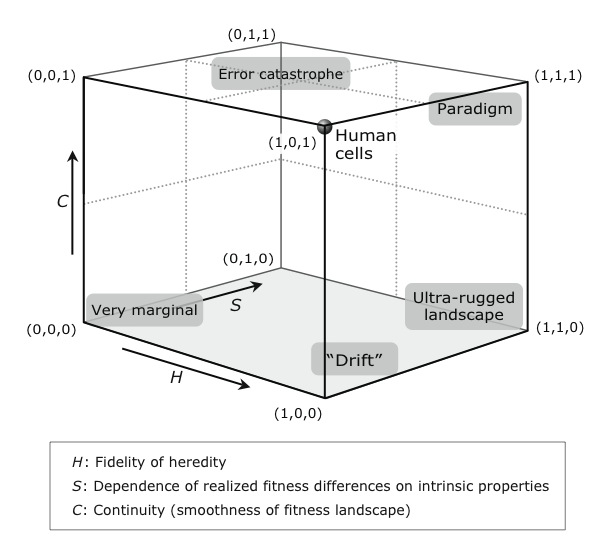
\includegraphics{./images/PGS.png}
	\end{center}
	\caption{L'espace tridimensionnel extrait de \citet[p.~64]{godfrey2009darwinian}}
	\label{fig:PGS}
\end{figure}

Selon l'auteur, cette décomposition des caractéristiques des populations par les différents facteurs qu'il propose n'est pas la seule possible. On pourra trouver d'autres caractéristiques importantes, les décomposer plus finement, ou même décomposer totalement différemment en fonction des besoins.  On pourra mettre en avant certaines caractéristiques pour éclaircir un cas précis et en considérer d'autres comme négligeable, puis inverser les hypothèses et changer la caractéristique centrale à étudier. D'ailleurs, l'auteur illustre la souplesse de cette approche en réfléchissant à ce qu'il appelle les <<\,reproducteurs collectifs\,>>. Pour attaquer l'étude de ces concepts il utilise d'autres caractéristiques qui lui permettent de mieux classer les populations qui correspondent à ces <<\,reproducteurs collectifs\,>>. Dans ces populations, les facteurs que nous avons évoqué précédemment sont déjà plus ou moins clairs et fixés, l'intérêt est déplacé sur d'autres dimensions de l'espace de PGS.

La vision de ce dernier permet donc de rendre compte du monde du vivant d'une façon assez complète:
\begin{quotation}
	Une [vision] dans laquelle les constituants du monde sont un large panel de populations darwiniennes: des cas paradigmatiques et des cas marginaux, certains clairs et d'autres obscurs, certains puissants et d'autre limités. Certains sont visibles et évidents, d'autre sont invisibles. Certains sont à l'intérieur d'autres. Ils avancent selon leur comportement darwinien suivant une large gamme d'échelles différentes, temporelles et spatiales. Certains évoluent via la reproduction d'un tout défini, d'autres évoluent en cooptant le matériel biologique qui en résulte [de la reproduction des premiers]. Les populations évoluent en fonction de leurs propriétés darwiniennes, mais changent aussi la base de leurs évolutions futures, en se déplaçant dans l'espace imaginaires de leurs paramètres évolutifs.\\
	\citep[p.~128]{godfrey2009darwinian}
\end{quotation}

Nous pensons que ce cadre de réflexion est l'outil idéal pour assurer le lien entre la Robotique \'Evolutionnaire et les recherches en Biologie car il permet de réfléchir à des cas d'évolution très différents tout en les situant sur un même continuum. Pour PGS ces cas ne sont pas de nature différente, et diffèrent juste de degré de certaines propriétés. Cela permet de lier entre eux des systèmes à première vue très différents les uns des autres, et de donner d'intéressantes pistes quant au chemin évolutif à suivre pour passer de l'un à l'autre.  Nous verrons comment ce cadre offre un moyen pratique pour positionner les recherches en Robotique et les comparer avec les connaissances des systèmes biologiques, tout en offrant aux chercheurs des indices sur les façons de construire leurs systèmes artificiels.


\section{Conclusion}
Dans cette partie nous avons essayé de montrer comment la théorie de l'évolution, telle que Darwin l'avait imaginée, est structurée et certains problèmes qu'elle a pu et peut encore rencontrer. Pour arriver à cette fin nous avons rapidement retracé l'histoire de cette théorie, en suivant le modèle de \cite{gayon1991darwinetlapresdarwin}. Nous avons notamment parlé des objections faites par Jenkin et comment ces objections ont amené les biologistes à utiliser l'outil statistique pour essayer de manipuler, comprendre et illustrer la théorie de l'évolution. Dans ce but nous avons présenté les travaux des biométriciens, pour ensuite décrire l'état actuel de la théorie en décrivant brièvement la vision la plus largement admise dans la communauté scientifique, amenée par la Synthèse Moderne que nous présentons dans ses (très) grandes lignes.

Nous avons ensuite essayé de montrer quelles pouvaient être aujourd'hui les questions qui agitent ces consensus, en illustrant les problèmes qui ont émergé et qui se sont cristallisés autour du débat sur les unités et niveaux de sélection. Sans nous prétendre exhaustifs, nous avons essayé de dégager quelques positions caractéristiques prises autour de ce débat, puis nous avons terminé en développant le cadre de réflexion de \cite{godfrey2009darwinian} dans lequel nous souhaitons positionner notre objet d'étude principal à savoir: la Robotique \'Evolutionnaire.

Cette mise au point théorique nous semble importante car elle permet \begin{inparaenum}[(\itshape\,1\,\upshape)]
\item de clarifier la théorie que reprennent l'algorithmique et la Robotique \'Evolutionnaire,
\item de souligner les limites et les objectifs de cette théorie,
\item de comprendre avec précision à quelles questions et quels problèmes un outil ayant pour but l'étude de la théorie de l'évolution va rencontrer et doit pouvoir répondre. 
\end{inparaenum}

Avant de décrire (dans la dernière partie) la Robotique \'Evolutionnaire et l'avancer comme un outil d'étude pour explorer cette théorie que nous venons de décrire, nous allons, dans la partie suivante, avancer d'autres outils théoriques et empiriques utilisés par les chercheurs et philosophes pour réfléchir et trouver des réponses aux débats qui remuent la biologie l'évolution tel celui présenté dans la partie \ref{sec:lvl}.
  %%Théorie de l'evolution, histoire principes, problèmes

\chapter{Méthodes d'études traditionnelles, modèles et simulations informatiques}\label{ch:methode}

\lettrine[lines=2]{C}{e chapitre} va être l'occasion de passer en revue différents outils d'investigation qu'utilisent les chercheurs pour étudier la théorie de l'évolution. Sans nécessairement prétendre être exhaustif, nous commencerons par analyser rapidement les méthodes plus <<\,traditionnelles\,>> que sont l'analogie et les expériences de pensée.

Dans une seconde partie nous nous attarderons sur les modèles et leur application dans le domaine de la biologie. Nous verrons comment ils peuvent être intégrés dans une vision générale de la science via notamment l'approche sémantique des théories \citep{vanfraassen1980thescientificimage,suppe1989thesemanticconceptionoftheoriesandscientificrealism} et l'intégration de la biologie de l'évolution dans cette conception de la science \citep{thompson1987adefenceofthesemanticconceptionofevolutionarytheory,lloyd1984asmanticapproachtothestructureofpopulationgenetics,beatty1980whatswrongwithreceivedwiew}.  

Nous analyserons enfin plus en détails les simulations informatiques et notamment celles mises au point par les chercheurs dans le domaine de la \emph{Vie Artificielle}. Nous verrons comment sont perçues ces simulations par les acteurs de cette discipline \citep{barandiaran06alifemodelsasepistemicartefacts} et nous reprendrons à notre compte leurs positions et leur classification.



\section{Modèles et simulations informatiques}\label{sec:cmpdr:va} 

\subsection{Les modèles}
Depuis le milieu du XXe siècle, la biologie tout comme les sciences dans leur ensemble, ont vu se démocratiser l'utilisation et l'application de \emph{modèles}. Ces derniers représentent, via des abstractions, des schémas, des équations, certains objets du monde, certaines parties, certaines entités des théories scientifiques. Ces représentations permettent de mieux étudier et comprendre les objets physiques ou théoriques, d'affiner et explorer les théories scientifiques. 

La place particulière des modèles dans la science est un sujet de philosophie des sciences \emph{en général} (de \emph{toutes} les sciences), et est donc très vaste. Quel est leur lien vis à vis du monde réel, comment s'articulent-ils avec les théories scientifiques et avec les expériences empiriques traditionnelles, quel statut ontologique leur donner,etc., sont autant de questions complexes qui présupposent de nombreuses mises au point et partis pris philosophiques que nous ne pouvons traiter ici.

Mais malgré toutes ces questions, aujourd'hui, il semble que les différentes écoles de pensée philosophiques :
\begin{quote}
	s'accordent toutes pour dire que les modèles sont des unités centrales de la construction de théories scientifiques.\\ \citep{frigg2012modelsinscience}
\end{quote}

Nous choisirons de suivre cette constatation. Pour le reste de notre exposé nous allons présenter une version naïve et simplifiée de la vue sémantique des théories qu'ont développé, entre autres, \cite{suppe1989thesemanticconceptionoftheoriesandscientificrealism,vanfraassen1980thescientificimage}, pour comprendre les sciences en général et qui permet d'intégrer ces modèles à une vision globale de la science.

Cette conception des théories scientifiques soutient que ces dernières (les théories scientifiques) sont mieux décrites par des familles de modèles que par des axiomes mathématiques logiquement articulés qui décrivent directement le réel, des <<\,lois de la nature\,>> (\,comme les lois de Newton\,). 

\cite{thompson1989thestructureofbiologicaltheories} ---qui reprend les auteurs cités précédemment, résume le rôle des modèle au sein de cette conception sémantique ainsi :

\begin{quotation}
	[Dans la conception sémantique] une théorie (un modèle) est une entité mathématique qui n'est pas définie par référence à un système formel. En d'autres termes ; bien qu'un système formel dans lequel la théorie sera vraie puisse être construit, la théorie (le modèle) n'est pas construite comme une interprétation d'un tel système formel. Elle est définie directement en spécifiant le comportement du système. Et, plus important, les lois ne décrivent pas le comportement d'objets du monde ; elles spécifient la nature et le comportement d'un système abstrait. Ce système abstrait, indépendamment de sa spécification, est déclaré comme isomorphe avec un système empirique particulier. \'Etablir cet isomorphisme nécessite d'autres théories scientifiques et l'adoption de méthodologies (comme les théories de design expérimental et de d'ajustement des modèles).\\
	\citep[p. 72]{thompson1989thestructureofbiologicaltheories}
\end{quotation}

Bas van Fraassen, lui, conclut :
\begin{quote}
	De ce point de vue, le travail essentiel d'une théorie scientifique est de nous fournir une famille de modèles, que l'on pourra utiliser pour représenter les phénomènes empiriques \citep{vanfraassen1972aformalapproachtothephilosophyofscience}.
\end{quote}

C'est cette naïve interprétation rapidement esquissée (chaque auteur en ayant en vérité une version qui lui est propre et bien plus complexe), que nous voulons reprendre pour la suite de notre exposé et qui nous semble adapté pour étudier la théorie de l'évolution.

Nous avons parlé rapidement, dans le chapitre précédant, des problèmes que la théorie de l'évolution peut poser. Nous avons notamment décrit dans la section \ref{sec:pgs} les commentaires que Godfrey-Smith a pu faire vis-à-vis de certaines descriptions et formulations de cette théorie (les <<\,recettes\,>>), et de ce besoin de construire un schéma général qui ne marche pas, ou des schémas particuliers qui ne généralisent plus. Il est à noter aussi, mais nous ne le détaillerons pas ici, que de nombreuses critiques ont souvent pointé du doigt la biologie comme une science qui ne possède pas de loi, puisque toutes les règles qu'elle a pu mettre au point (lois de Mendel, équilibre de Hardy-Weinberg), présentent de nombreuses exceptions. Nous avons vu comment PGS intègre ces exceptions dans son espace : il construit un modèle qu'il veut souple, qui peut être déformer pour intégrer les différentes composantes et leurs exceptions. 

C'est pour répondre à ces incohérences, pour justifier le besoin de multiples modèles et asseoir la valeur scientifique de ces modèles biologiques dans une vision globale de la science, que \cite{beatty1980whatswrongwithreceivedwiew,beatty1980ptimaldesignmodelsandstrategyofmodelbuildinginevolutionarybiology,beatty1987onbehalfofsemanticview,thompson1989thestructureofbiologicaltheories,thompson1987adefenceofthesemanticconceptionofevolutionarytheory,lloyd1984asmanticapproachtothestructureofpopulationgenetics,lloyd1988thesemanticapproachanditsapplicationtoevolutionarytheory}, ont repris la conception sémantique des théories pour l'appliquer à la biologie et en particulier à la biologie de l'évolution.

Ainsi, si \cite{beatty1980whatswrongwithreceivedwiew} considère qu'il ne peut effectivement pas y avoir de loi au sens classique des théories (des <<\,lois de la nature\,>>), puisque, par exemple, les lois de Mendel, ou l'équilibre de Hardy-Weinberg, sont le fruit du processus évolutionnaire et sont toujours soumis à son action :
\begin{quote}
	C'est à dire que les théories évolutionnaire peuvent changer en tant que [elles sont le] résultat du changement évolutionnaire \citep[p.~407]{beatty1980whatswrongwithreceivedwiew}.
\end{quote}
Ceci n'est plus un problème à la lumière de la conception sémantique des théories. Comme nous l'avons déjà dit, suivant cette conception, les faits empiriques sont indépendants de la théorie et des modèles qui la composent. Ainsi, qu'importe si certains systèmes empiriques ne suivent pas l'équilibre traditionnel de Hardy-Weinberg et nécessitent une version améliorée et différente de celui-ci : les populations qui respectent l'équilibre classique seront décrites par la théorie tout comme celles qui nécessitent un modèle plus complexe \citep[p.~410-411]{beatty1980whatswrongwithreceivedwiew}.
Cette vision des théories scientifiques s'articule très bien avec notre volonté d'étudier la biologie à travers le prisme de modèles évolutionnaires robotiques (ou plutôt, notre volonté s'articule très bien avec la conception sémantique). Différents modèles de Robotique \'Evolutionnaire pourront décrire différents systèmes biologiques, sans qu'il soit nécessaire que le modèle robotique décrive une \emph{loi de la nature}. Et même si la plupart des auteurs que nous avons cités considèrent souvent les modèles comme des entités mathématiques formels, il y en a pour penser qu'ils peuvent être <<\,des modèles caractérisés non mathématiquement\,>>\citep[p. 1]{lloyd1988thesemanticapproachanditsapplicationtoevolutionarytheory}. Nous pensons et nous allons essayer de montrer, que les simulations informatiques peuvent elles aussi être perçu comme des modèles solides et intéressants, qui présentent de nombreuses propriétés particulières utiles pour comprendre la théorie de l'évolution.

\section{Conclusion}
Dans ce chapitre nous avons rapidement présenté quelques méthodes utilisées par les chercheurs pour étudier la théorie de l'évolution et essayer de résoudre les problèmes qu'elle génère. Nous avons d'abord parlé de la sélection artificielle et de son utilisation par Darwin puis, comment cette idée d'étudier des entités physique soumises à des pressions sélectives artificielles dans des <<\,expériences\,>> de laboratoire a perduré et quel est l'intérêt de ce type d'expériences. Nous avons ensuite brièvement parlé des expériences de pensée, pour introduire des méthodes laissant plus de libertés aux expérimentations et tests possibles.
Dans la deuxième partie de ce chapitre nous avons parlé des modèles en essayant de justifier leur utilisation en sciences via la conception sémantique des théories scientifiques. Nous avons soutenu l'intérêt de l'utilisation de la simulation informatique comme modèle et donc leur importance au sein la conception sémantique. 

Pour mieux cerner l'intérêt de ces simulations afin d'étudier la biologie, nous avons repris les analyses des chercheurs en Vie Artificielle en détaillant les modèles épistémiques conceptuels et leur liens avec les expériences de pensée. Nous pensons que ces modèles offrent la plus grande liberté de mano\oe uvre pour travailler sur la théorie de l'évolution, et nous verrons dans la dernière partie de ce mémoire un type de simulations qui tombent, selon nous, dans cette catégorie tout en essayant de s'affranchir de certaines limites évoquées dans ce chapitre.

L'objectif principal de cette partie a été de dégager certains avantages et inconvénients des méthodes décrites. Nous avons vu que certaines méthodes, comme l'analogie avec la sélection artificielle des éleveurs ou l'évolution dirigé de Lenski, essaient de se rapprocher le plus possible des expériences empiriques traditionnelles en fournissant des résultats directement applicables à la théorie de l'évolution des êtres vivants. Néanmoins ces méthodes souffrent de certaines difficultés techniques dues notamment aux contraintes imposées par le vivant. Ainsi, d'autres méthodes essayent d'abstraire les propriétés des êtres vivants via des expériences de pensées ou des simulations, dans le but de s'offrir une plus grand liberté d'études. En contrepartie, l'application des résultats obtenues par ces méthodes à la biologie requiert plus de précautions et peut parfois être un véritable problème, voir impossible.
 %%étudier la théorie de l'évolution : expériences de pensée, modèles, simulation


\chapter{La Robotique \'Evolutionnaire}\label{ch:RE}

\lettrine[lines=2]{N}{ous} terminerons ce mémoire en décrivant en détails la Robotique \'Evolutionnaire. Nous commencerons par rappeler son histoire et ses influences, puis nous décrirons dans les grandes lignes la méthodologie traditionnelle de la discipline.

Nous verrons ensuite certains problèmes que cette méthodologie implique et introduirons les voies suivies par certains chercheurs pour essayer de les résoudre. Nous insisterons sur l'\emph{\'Evolution Embarquée} \citep{watson02embodiedevolutiondistributingevolutionaryalgorithmpopulationrobots} et \emph{dirigée par l'environnement} \citep{bredeche2012environmentdrivendistributedevolutionaryadaptation}, car, et nous verrons pourquoi, ces dernières nous semblent les développements de la Robotique \'Evolutionnaire les plus appropriés pour étudier la biologie.

\section{Histoire et principes}\label{sec:re}
\subsection{Bref Historique}
\label{sec:re:hist}


Comme nous l'avons déjà décrit en introduction, la Robotique \'Evolutionnaire (RE, en anglais ER, \emph{Evolutionary Robotics}) descend directement de l'Algorithmique Évolutionnaire. Le principe clef est de reprendre <<\,l'outil\,>>, les \emph{recettes} (comme les appelle \cite{godfrey2009darwinian} cf. section \ref{sec:pgs}) de la théorie darwinienne de l'évolution revue et corrigée par les néo-darwiniens et la synthèse moderne, afin de trouver une méthode pour construire automatiquement des robots.
Comme nous l'avons aussi déjà introduit, l'intuition que l'évolution selon Darwin peut s'appliquer à des machines pour leur offrir la complexité et la robustesse nécessaires à leur autonomie dans le monde réel est aussi vieille que l'informatique elle-même, le texte de \cite{turing50computingmachineryintelligence} en faisant foi.

Mais bien que cette intuition fût présente alors que l'informatique balbutiait au stade embryonnaire, il a fallu attendre : 1. l'invention de l'Algorithmique \'Evolutionaire (AE, cf. \ref{sec:intro:ae}) pour démontrer le bien fondé et l'utilité de l'application de ces idées à des entités numériques ; et, 2. qu'émerge une nouvelle école de robotique aux fondements théoriques différents de la robotique classique en vigueur aux débuts de l'AE pour que l'intuition de Turing trouve un terrain empirique et théorique fertile à son implémentation.

Nous avons déjà vu en introduction les principes et l'histoire de l'algorithmique évolutionnaire et avant d'en faire de même pour la Robotique \'Evolutionnaire (RE), prenons le temps de dire deux mots sur ce qui nous semble le second prérequis à la naissance de la RE, c'est à dire : \emph{l'apparition d'une nouvelle école en robotique}.

Ce nouveau courant, dont la portée peut en fait être étendue à l'Intelligence Artificielle en général, a opéré un changement conceptuel quasi philosophique à la fin des années 80. Les roboticiens de cette période ont démontré que la voie suivie par l'Intelligence Artificielle traditionnelle de l'époque, fille du computationalisme des années 60, n'était pas la seule possible. Reprenant les travaux de \citet{braintenberg86vehicles} et de certains éthologues, \cite{brooks91intelligencewithoutreason}, notamment, montra que pour obtenir des comportements efficaces et robustes\footnote{Nous entendons par robuste : peu sensible aux conditions initiales} dans des environnements complexes, la longue computation d'une représentation symbolique du monde n'est pas forcément la meilleure solution pour agir avec justesse et rapidité. Souvent, il suffit de construire un système dont les propriétés morpho-physiologiques répondent correctement aux contraintes de l'environnement, capable de s'imbriquer dans une boucle <<\,perception-action\,>> simple et <<\,réactive\,>> (la robotique issue de ces réflexions étant bien souvent appelée <<\,Robotique Réactive\,>>).

Ce changement de perspective paraît <<\,plus en accord avec l'histoire évolutive des organismes\,>> \citep[Brooks dans la préface de ][p. 15]{pfeifer2006howthebodyshapesthewaywethink}. Il débarrasse ainsi l'intelligence de la complexité du computationalisme et permet aux chercheurs en évolution artificielle d'imaginer pouvoir coder simplement des comportements efficaces et intéressants, sans besoin de bases de données gigantesques manipulées par des systèmes experts complexes.

Il est à noter qu'à la même époque les neurones formels, initialement introduits par \cite{mcculloch1943alogicalcideaimmanervacti}, étaient en plein développement. En particulier, au milieux des années 80, \cite{rumelhart1986learninginternalrepresentationsbyerrorpropagation} inventaient un type particulier de réseaux de neurones formels, les perceptrons multicouches. Nous reparlerons en détail de ces réseaux un peu plus tard dans cette partie, soulignons juste pour le moment que ces outils computationnels, apparus au bon moment, se sont révélés un modèle parfait pour implémenter le paradigme de Brooks, et deviendront un élément central de la Robotique \'Evolutionnaire. Leur utilisation et leur principe de fonctionnement (que nous reverrons) les rendent assez simples pour qu'ils puissent être largement utilisés tout en présentant des caractéristiques essentielles aux études de RE (nous verrons lesquelles plus tard).

La naissance de la Robotique \'Evolutionnaire eut lieu de façon quasi simultanée et en parallèle dans trois universités différentes au début des années 1990. Une en Angleterre dans la ville de Sussex, une aux Etats Unis à l'université de Caroline du Sud, et l'autre en Suisse, à l'Ecole Polytechnique Fédérale de Lausanne (cf la préface de \cite{nolfi00evolrobobiolintetechselfmach} ou encore \citet{harvey97evolutionaryroboticssussexapproach} pour une introduction plus détaillée de cette naissance vue par l'école anglaise).

Dès le début l'application de ces méthodes pour étudier la biologie --application que nous voulons défendre ici, était envisagée par les fondateurs de la discipline. Ainsi, \cite{cliff93explorationsinevolutionaryrobotics} expliquent dès le résumé d'un article d'époque qui passe en revue leurs premières avancées dans le domaine, que si leur objectif premier <<\,est de développer des systèmes de contrôle sensorimoteur pour des robots mobiles, [ils veulent] aussi discuter l'applicabilité de [leur] approche à l'étude des systèmes biologiques.\,>> \citep[p. 73]{cliff93explorationsinevolutionaryrobotics}. De même ils se considèrent plus proches de <<\,la neuroethologie que des neurosciences computationnelles\,>> (\emph{ibid.} p. 74) ; neurosciences computationnelles qui sont la source d'inspiration première de la robotique classique, quand la robotique de Brooks est elle plus proche de l'ethologie.

Cette proximité avec la biologie se retrouvera tout au long de l'histoire de la Robotique \'Evolutionnaire. Le but avoué est bien de développer des techniques automatiques pour <<\,construire des robots autonomes intelligents et comprendre comment les animaux sont ``construits''\,>>(\emph{ibid.}, guillemets d'origine). La RE s'est donc très vite positionnée comme une discipline proche de la Vie Artificielle, qui était à l'époque des premiers travaux de Robotique \'Evolutionnaire en pleine effervescence \citep{langton89alifeiproceedingsfirstinternationalworkshopsynthesissimulationlivingsystems}. Ainsi, contrairement à l'algoritmique évolutionnaire qui a assez vite pris de la distance vis a vis de son inspiration biologique originelle, les buts et directions de la Robotique \'Evolutionnaire sont restés intimement liés à ce désir d'être à la fois un outil \emph{inspiré par} la biologie, mais aussi \emph{inspirant pour} la biologie.

Les roboticiens ont bien compris et repris l'idée de \cite{maynardsmith78optimizationtheoryinevolution} dont nous avons déjà parlé en introduction en introduction, pour la reformuler selon leurs termes :
\begin{quotation}
   Il y a une similarité entre le problème d'ingénierie de créer un robot autonome fonctionnel amené à agir dans un environnement complexe et bruité et le problème scientifique de proposer un modèle plausible des mécanismes sous-jacents la genèse du comportement adaptatif d'un animal.\\
   \citep[p. 74]{cliff93explorationsinevolutionaryrobotics}
\end{quotation}

De même pour \citet[p. 12-13]{nolfi00evolrobobiolintetechselfmach}, la question principale motivant la RE est de permettre de comprendre :
\begin{quotation}
   Quelles sont les caractéristiques clefs de l'évolution naturelle qui la rendent capable de produire l'extraordinaire variété de formes de vie hautement adaptées présentes sur la planète? Répondre à cette question pourrait améliorer significativement à la fois notre compréhension des systèmes biologiques et notre habilité à concevoir des systèmes artificiels.
\end{quotation}

Assez vite une communauté va se former autour des groupes de Sussex, de l'USC et de l'EPFL. Cette communauté va réunir des chercheurs en Vie Artificielle, en Robotique, en \'Ethologie, en Algorithmique \'Evolutionnaire ou encore en Neurosciences Cognitives. De nombreuses études vont être menées, s'appuyant sur des approches différentes, avec des ambitions différentes, mais ayant toutes un ensemble de problématiques et de méthodes similaires. Puis en 2000 parait le livre <<\,éponyme\,>> \emph{Evolutionary Robotics} \citep{nolfi00evolrobobiolintetechselfmach}. La publication de ce livre quelques années après la première conférence entièrement consacrée au sujet en 1998 peut être perçue comme l'auto-reconnaissance de la Robotique \'Evolutionnaire en tant que discipline à part entière. En publiant cet ouvrage elle n'est plus simple sous  composante de telle ou telle autre discipline, mais devient une discipline en tant que telle, maitresse de ses propres buts et utilisant ses propres méthodes.

Voyons maintenant plus en détails les éléments et outils qu'elle mobilise.

\subsection{Méthodes et Principes}
\label{sec:re:meth}

Le principe de base de la Robotique \'Evolutionnaire (RE) est exactement le même que celui que nous avons présenté en introduction pour décrire l'Algorithmique \'Evolutionnaire (AE) : appliquer les principes de l'évolution selon Darwin à des artefacts humains (plus précisément numériques dans le cas de l'AE).

Parmi les différences notables (que nous avons déjà soulevées) entre AE et RE, les premières à s'imposer sont : l'objet, la nature de l'objectif et l'environnement avec lesquels travaillent les roboticiens. Le but de ces derniers est de construire des robots qui doivent se déplacer de façon tout à fait autonome dans des environnements <<\,réels\,>>, qu'on ne connait pas forcément à l'avance. Ces environnements sont susceptibles de subir de nombreux changements pendant l'activité du robot, changements qui peuvent (et qu'on peut souhaiter) être produits par le robot lui-même. Les contraintes qui s'appliquent sont donc beaucoup plus proches de celles auxquelles sont soumis les êtres vivants que des solutions et des objets manipulés par l'AE.

Néanmoins une limitation technologique importante, qui diminue de beaucoup l'étendue de l'analogie possible entre RE et biologie apparait d'emblée et doit être soulignée et soulignée et  prise en compte au plus tôt. La grande majorité des travaux, et la quasi totalité des méthodes que nous allons décrire, portent sur le développement par évolution artificielle des éléments responsables du contrôle des <<~enregistrements~>> (les perceptions, les données reçues par les capteurs) et des déplacements des robots. En d'autres termes : les régulateurs de la boucle sensorimotrice <<\,perceptions/actions\,>> ---ce qui pourrait correspondre, si l'on poursuit quand même l'analogie, au système nerveux des êtres vivants, dont la partie visible par l'observateur est ce qu'on pourrait appeler le \emph{comportement} des robots. La morphologie des robots quant à elle n'est en aucun cas modifiée. Elle est fixe et imposée dès le départ par le modèle de robot choisi pour l'étude en question et ne changera pas, si ce n'est à cause de problèmes d'usure.

Or dans le monde du vivant, l'évolution du système nerveux est intimement liée à l'évolution de la morphologie des êtres biologiques qu'il <<\,contrôle\,>>. Plus encore, depuis une vingtaine d'années un grand nombre d'études et quasiment toute une école de pensée (souvent désignée par le terme de \emph{embodied cognition} et qui est d'ailleurs elle aussi une descendante directe des changements de perspective en robotique dont nous avons parlés précédemment) tendent à montrer que cette coévolution est essentielle pour qu'émergent les fonctions cognitives <<\,avancées\,>> qu'ont pu développer, par exemple, les poulpes \citep{pfeifer2006howthebodyshapesthewaywethink}. Néanmoins ce découplage de l'évolution du comportement et du corps ne doit pas empêcher d'appliquer les méthodes d'évolution artificielle à l'étude de l'évolution en général.

Premièrement, ce découplage n'a pas empêché les chercheurs du domaine de rapidement le cerner comme une limite. Au contraire, nombreuses sont les études en RE et plus largement en AE appliquée à des systèmes électroniques, qui ont mis en avant l'importance du couplage morphologie/contrôle sensorimoteur. Le rôle de ces expériences est très certainement central dans la prise de conscience de l'importance de ce problème chez les acteurs de la communauté. Et ils s'accordent aujourd'hui tous sur le fait que :
\begin{quote}
	[\ldots] ce n'est pas ainsi que l'évolution naturelle agit. L'évolution ne démarre pas avec un corps donné et ensuite fait évoluer un cerveau pour ce corps ; en revanche, les deux, corps et cerveau, évoluent ensemble au cours du temps. Pour des systèmes artificiels, la capacité de faire évoluer la morphologie et le contrôle neuronal de concert est cruciale si nous voulons exploiter la totale puissance de l'évolution.
   \\\citep[p. 193]{pfeifer2006howthebodyshapesthewaywethink}
\end{quote}

De plus, forts de cette constatation, les chercheurs ont proposé des solution pour pallier ce problème.  Parmi les premières et les plus connues il y a les remarquables expériences de \cite{sims1994evolving3dmorphologyandbehaviorbycompetition}. Ce dernier a, avec succès, fait coévoluer morphologies et comportements dans des simulations avec des résultats aussi étonnants que convaincants\footnote{Des vidéos et plus de détails sur ces expériences sont disponibles ici : \\ http://www.karlsims.com/evolved-virtual-creatures.html.}. Ces expériences ont été suivies par celles de \cite{pollack2000thegolemproject} dans lesquelles les auteurs ont voulu donner une forme physique aux simulations de Sims, ou encore dans les travaux de \citet[ch. 6]{pfeifer2006howthebodyshapesthewaywethink}.
Cet effort est toujours à l'œuvre et reste un des objectifs centraux de la discipline (la <<\,synthèse automatique\,>> comme la nomment \cite{doncieux2009exploringnewhorizonsinevolutionqryrobotics}). L'idée est de laisser à l'évolution le soin de modeler un maximum d'éléments des agents à concevoir et de minimiser le plus possible l'intervention de l'humain. Cette volonté est très présente dans les nombreuses tentatives de rapprochement de la RE avec les sciences du développement en biologie pour former ce que certains appellent <<\,l'evodevorobo\,>> \citep{bredeche11evolutionaryadaptationpopulationrobots} et qui fait dire à \citet[p. 17]{nolfi00evolrobobiolintetechselfmach} que le <<\,développement est une des issues les plus débattues en Robotique \'Evolutionnaire\,>> et que:
\begin{quote}
	La direction la plus prometteuse [en Robotique \'Evolutionnaire] est d'inclure dans le processus évolutionnaire d'autres mécanismes tel que la plasticité ontogénique qui pourrait augmenter la puissance adaptative du processus évolutionnaire sans accroitre le rôle du concepteur humain.
	\\(\emph{ibid.})
\end{quote}

En dernier point il est à noter que ce découplage n'enlève pas nécessairement la valeur que peuvent avoir certains modèles de RE. Malgré les abstractions  qui doivent être faites lors des expériences de RE, si ces dernières présentent certaines caractéristiques essentielles similaires à certaines situations biologiques particulières, la simulation peut apporter des informations sur la compréhension du pendant biologique de l'expérience de robotique. De plus, ce découplage, cette distinction comportement/morphologie que semble imposer la RE est vrai si on considère que l'analogue du <<\,corps\,>> des individus biologiques est la structure matérielle du robot et que l'individu artificiel est le couple $(Programme,Robot)$. Or cette analogie, bien que peu discutée car découlant directement de la façon dont sont implémentés les algorithmes évolutionnaires en RE, n'est peut-être pas la plus adéquate. Elle le semble d'autant moins lorsque l'on considère l'important développement des méthodes de <<\,swarm intelligence\,>> par de nombreux chercheurs de la discipline. Dans ces études, les scientifiques font évoluer des populations de robots capables de s'associer et de se spécialiser, dans lesquelles la distinction entre individus/morphologies/robots/populations n'est plus si claire.

Une fois apportées ces précisions, essayons de nous pencher plus en détail sur le fonctionnement des algorithmes évolutionnaires utilisés en RE.

Dans sa version la plus classique, une expérience de Robotique \'Evolutionnaire se déroule comme suit \citep[pour certains exemples historiques de la littératures]{nolfi96learning,floreano94automaticcreationofanautonomousagen,jakobi97evolutionaryroboticsandtheradicalenvelopeofnoisehypothesis}:

\begin{inparaenum}[(\itshape 1\upshape)]

D'abord, \item \label{it:deftache}, une tâche que le robot doit résoudre est définie (prenons par exemple la tâche de ramener un objet dans le coin précis d'une pièce, repéré par une couleur particulière). Ensuite, \item, \label{it:choixctrl} un type de contrôleurs, les programmes informatiques qui vont s'occuper de gérer le comportement du robot, doit être choisi.
\\ 
Ces contrôleurs doivent avoir des propriétés particulières pour que l'algorithme évolutionnaire fonctionne:

   \begin{inparaenum}[(\itshape a\upshape)]
   En premier lieu, ils doivent, \item fournir aux robots les capacités (que nous pourrions, dans notre cas, qualifier de <<\,cognitives\,>>) nécessaires à l'accomplissement de la tâche. Par exemple : si le robot doit parcourir un labyrinthe complexe dans lequel il doit trouver une sortie, alors le robot doit être capable de mémoriser les lieux qu'il visite. Le contrôleur doit pouvoir offrir et gérer cette mémoire.
   Dans un second temps,\item, sachant que c'est le contrôleur le responsable du comportement du robots, c'est lui qui va être soumis à l'évolution. C'est lui qui va <<\,subir\,>> les mécanismes nécessaires à l'évolution. Il va être répliqué, muté, croisé,\ldots. Il faut donc que le contrôleur utilisé puisse supporter ces opérations. Tout comme dans le cas du voyageur que nous avons vu dans l'\ref{sec:intro:vc}introduction, où il était possible de représenter la solution par une chaine de caractères que l'on pouvait aisément muter et croiser, le contrôleur du robot doit présenter des propriétés similaires.
   \end{inparaenum}
   Une solution souvent adoptée par les chercheurs est, comme nous l'avons déjà rapidement sous-entendu, l'utilisation de réseaux de neurones artificiels (RNA \emph  {Artificial Neural Network},  en anglais). Nous reviendrons plus en détails sur ces réseaux de neurones après. %%\label{it:RNA}

  Une fois ces contrôleurs choisis,  une <<\,population initiale\,>>, souvent appelé G0 pour reprendre une terminologie de biologiste, est générée, \item. Dans une expérience classique menée avec des réseaux de neurones artificiels, un nombre \emph{n} d'individu (de réseaux de neurones), va être construit (avec \emph{n} donnée arbitrairement \emph{a priori}, en fonction des moyens du laboratoire, de la patience du chercheur, etc.). Sachant que les réseaux de neurones peuvent être résumé (encodés) par des chaines d'entier, on aura donc, à l'issu de cette phase d'initialisation, \emph{n} chaines d'entier obtenues aléatoirement. \label{it:init}

 \item Ces contrôleurs générés aléatoirement doivent ensuite être testés sur les robots. Pour cela, différentes méthodes sont possibles. Nous en verrons d'autres, mais la classique et historique méthode utilisée par les pionniers de la discipline (aux moyens limités et qui ne possédaient qu'un robot) est la suivante: chaque contrôleur est envoyé sur l'unique robot puis exécuté. Lors de l'exécution du contrôleur, un certain nombre de données qui serviront à déterminer le degré de réussite du robot sont enregistrées. Une fois l'exécution terminé, le contrôleur est stocké conjointement avec les résultats obtenus lors de son exécution. Ensuite un autre contrôleur est chargé sur le robot pour être testé à son tour. Pour que la comparaison soit possible, il faut évidemment que les conditions initiales soient les mêmes, c'est pourquoi le robot doit être remis à son point de départ et toutes les conditions environnementales réinitialisées à l'identique. Ce travail de test est un travail long, fastidieux, sujet à beaucoup d'erreurs et loin de trouver un équivalent dans le monde biologique. Nous verrons certains méthodes qui contournent ce problème, notamment à travers ce que nous présenterons comme l'Évolution Embarquée (EE, cf \ref{sec:RE:EE}). \label{it:test}

 \item Une fois les tests de chaque contrôleur terminés, une mesure de leur réussite doit être faite pour qu'une comparaison qualitative entre les différents programmes puisse avoir lieu. C'est ce qu'il est convenu d'appeler la \emph{fonction fitness}. Cette mesure est un calcul qui va nous offrir le degré d'adaptation, donc la fitness du contrôleur, par rapport à la tâche à accomplir. En général un ensemble de variables (environnementales, <<\,physiologiques\,>>) enregistrées pendant l'expérience sont utilisées pour ce calcul. Par exemple, dans le cas de notre balle qui doit être ramenée dans un coin de labyrinthe, une bonne mesure peut être la distance restante entre la balle et l'objectif, distance que l'on pourrait pondérer par le temps mis et/ou la distance parcourue pour amener la balle à cette endroit. \label{it:fitness}

 \item \label{it:select} En fonction des résultats, un certain nombre de contrôleurs vont être sélectionnés. Cette sélection peut se faire en utilisant par exemple ce qu'il est convenu d'appelé la roulette proportionnée\footnote{Dans la roulette proportionnée les individus sélectionnés vont l'être de sorte que plus les individus ont une fitness élevée, plus ils ont de chance d'être sélectionnés. Ainsi on aura en moyenne les meilleurs individus dans les générations suivantes sans pour autant empêcher les individus les moins bons de transmettre leurs caractéristiques.}, mais ici encore d'autres méthodes peuvent être employées. Après cette étape de sélection nous allons, \item \label{it:reproduction} muter et croiser les <<\,solutions\,>>, les <<\,individus\,>> pour en obtenir de nouveaux. Ces nouvelles \emph{pseudo}-solutions constitueront une nouvelle génération, et l'expérience pourra repartir en \ref{it:test}.
\end{inparaenum}

La suite d'instructions que nous venons de décrire est un algorithme évolutionnaire, du même type que ceux utilisé pour résoudre le problème du voyageur de commerce vu en introduction. Appliqué à la robotique ils sont le cœur de la RE. 

En voici une version résumée:

\begin{algorithm}
	\dontprintsemicolon 
	\caption{Un Algorithme classique de Robotique \'Evolutionnaire}\label{alg:RE}
		 Définition de la tâche (\ref{it:deftache})\;
		 Choix des contrôleurs (\ref{it:choixctrl})\;
		 Initialisation de la génération G0 (\ref{it:init})\;
		\While{Expérimentateur \neq satisfait}{
		 Test des contrôleurs (\ref{it:test})\;
		 Calcul de la fitness (\ref{it:fitness})\;
		 Sélection (\ref{it:select})\;
		 Reproduction (mutations,croisements) \& création d'une nouvelle génération (\ref{it:reproduction})\;
	 }
\end{algorithm}

Évidement ce schéma, fortement inspiré de la biologie, peut-être raffiné et complexifié à loisir. Chaque étape peut être pensée et réalisée de multiples façons et est le sujet de projet de recherche à part entière. Certaines de ces étapes vont poser plus de problèmes que d'autres et les résultats obtenus à l'issu de l'exécution de l'algorithme dépendrons beaucoup des choix faits. Nous avons déjà suggéré que le type de contrôleurs utilisés peut faire l'objet de ce genre de choix, il en est de même pour la façon de calculer la fitness, pour le type et le nombre de robots utilisés, l'utilisation de la simulation ou encore la manière de croiser et muter les individus. Tous ces paramètres sont autant d'éléments qui peuvent varier d'une étude à l'autre. La littérature abonde sur les pourquoi et comment choisir ces paramètres (cf  \cite{nolfi00evolrobobiolintetechselfmach} pour plus d'informations sur le sujet). Dans le cadre de ce travail, après avoir décrit un peu plus en détails les contrôleurs les plus utilisés et les raisons de cette utilisation, nous verrons des variations particulières parmi certains de ces choix méthodologiques. Nous insisterons particulièrement sur des variations qui permettent, selon nous, de dépasser certains obstacles de la RE traditionnelle et qui la rendent encore plus adéquate pour l'utilisation que nous souhaitons promouvoir ici, à savoir l'étude de la théorie de l'évolution.


\subsection{Les réseaux de neurones artificiels}\label{sec:RNA}

Comme nous l'avons annoncé au point \ref{it:choixctrl} de la description de l'algorithme évolutionnaire classiquement utilisé en RE, la plupart des chercheurs du domaine utilisent des réseaux de neurones artificiels.

Un réseau de neurones artificiels est un concept mathématique qui permet de relier des variables d'<<\,entrée\,>> à des variables de <<\,sortie\,>>. Plus explicitement, suivant une vague analogie avec la biologie, un neurone va recevoir une ou plusieurs données en entrée qui pourront être fournies par l'environnement ou par d'autres neurones, et va s'activer ou non en fonction des valeurs d'entrées et d'une fonction d'activation interne au neurone. À l'intersection entre les neurones (ou entre un neurone et un capteur) sont présentes des <<\,synapses\,>>. Ces synapses possèdent un poids, souvent susceptible de varier au cours de la vie d'un agent (c'est la base de l'<<\,apprentissage\,>>).

Sans nous attarder trop sur les détails de ces réseaux de neurones artificiels, rappelons rapidement que ceux-ci reprennent des concepts développés par \citep{mcculloch1943alogicalcideaimmanervacti} et sont faits en superposant des <<\,couches\,>> de neurones formels (les sorties des neurones des premières couches serviront d'entrée pour les neurones des couches suivantes). En règle générale, il est fréquent d'utiliser un type particulier et bien connu de neurones formels : les perceptrons. La mise en réseaux de ces perceptrons dans ce qu'il est convenu d'appeler par le terme technique des Perceptrons Multi-Couches (PMC, ou MLP pour \emph{Multi-Layer Perceptron} en anglais) offre une solution aux chercheurs en RE avec plusieurs avantages, ce qui en fait le candidat idéal des expériences évolutionnaires. Premièrement, il va être possible de relier les entrés du PMC aux différents capteurs du robots (capteurs de vitesse, infra-rouge, ultra-son, caméras, thermomètres, gyroscopes) et ses sorties sur les <<\,effecteurs\,>> du robot (moteurs, émetteurs lumineux). Ensuite, pour peu qu'on construise ces réseaux de façon adéquate et qu'on leur fournisse des règles pour le faire, ils vont pouvoir être soumis à un apprentissage \citep[p. 30-39]{nolfi00evolrobobiolintetechselfmach}. Cet apprentissage peut être mené de différentes façons à différentes étapes de l'algorithme. Soit pendant la <<\,vie\footnote{Ce qu'on désigne en général par la <<~vie~>> du robot est la période pendant laquelle le robot est testé, ce qui correspondrait à l'étape \ref{it:test} de l'algorithme évolutionnaire décrit précédemment.}\,>> du robot soit pendant une phase spécifique d'apprentissage. Ces méthodes offrent au robot une <<\,mémoire\,>> et donc la possibilité pour lui de résoudre des tâches plus complexes. Pour terminer avec ce qui nous semble être les principaux atouts des réseaux de neurones artificiels, ces derniers peuvent être très simplement représentés en résumant chaque neurone par le poids de ses <<\,synapses\,>>, la fonction d'activation et les règles d'apprentissage dont il va se servir. Ainsi, ce qui sera considéré comme notre <<\,individu\,>>, soumis à l'évolution, sera une chaîne de nombres, codant pour des poids et des fonctions mathématiques qui seront utilisés dans un Perceptron Multi-Couches conçu pour contrôler un robot.

De façon plus exhaustive et détaillée que ce que nous venons de faire, \citet[p. 39]{nolfi00evolrobobiolintetechselfmach} listent six caractéristiques indépendamment susceptibles de justifier l'emploi des RNA.
\begin{enumerate}
   \item Un \emph{espace de recherche lisse} : ce qui signifie qu'un changement léger dans les paramètres du réseau de neurones aboutira à un changement léger dans le comportement du robot.% Ce n'est pas exactement le paramètre C de PGS que nous avons évoqué dans la section \ref{sec:pgs} puisque la fitness n'entre pas directement en compte. Mais comme cette (? manque un mot) elle en est une composante certaine, d'autant plus que la fitness des robots est souvent assez directement corrélée à leur comportement. Il est intéressant de noter comme les roboticiens ont réalisé l'importance de cette condition (quelle condition?) pour que l'évolution soit possible.
   \item Les réseaux de neurones permettent d'ajuster une certaine \emph{granularité}: on peut, dans l'algorithme évolutionnaire mis en place, choisir de prendre en compte et faire évoluer uniquement les poids des neurones ou des groupes de neurones.
   \item Ils peuvent montrer \emph{différents niveaux d'adaptation} : phylogénétiques (évolution du poids des synapses au cours des générations), développementaux (maturation des connexions entre les neurones à l'initialisation des robots), ontogénique (apprentissage par renforcement, ou autre, avec modification des poids synaptiques au cours de la vie du robot).
   \item Ils offrent une \emph{correspondance directe entre senseurs et effecteurs} : les réseaux de neurones peuvent sans problème recevoir un signal d'entrée analogique continue depuis les capteurs et délivrer un signal discret ou continu aux moteurs selon les besoins.
   \item Ils sont relativement robustes au bruit. Même si les signaux délivrés par les capteurs sont bruités, étant donné que les données sont intégrées par des fonctions d'activation qui somment de nombreuses entrées pondérées, ils sont peu sensibles aux oscillations dûes au bruit d'une entrée.
   \item Ils sont une métaphore biologiquement plausible des mécanismes qui supportent les comportements adaptatifs. Ils se présentent donc comme un choix naturel pour qui veut comprendre et reproduire les comportements biologiques. \\
       \citep[Liste plus ou moins librement adaptée de ][p. 39 les emphases ont toutes été ajoutées]{nolfi00evolrobobiolintetechselfmach}
\end{enumerate}
\section{Challenges et méthodes alternatives, \'Evolution Embarquée}\label{sec:RE:EE}
\subsection{Challenges et obstacles}\label{sec:RE:EE:obs}
Mais comme nous l'avons évoqué, certaines étapes présentent des difficultés et les expériences en Robotique \'Evolutionnaire font face à de nombreux obstacles. \cite{mataric96challengesinevolvingcontrollersforphysicalrobots} essayaient déjà de les lister dans un article des débuts de la RE. Nous allons essayer d'en illustrer quelques uns en reprenant l'exemple que nous avons esquissé dans la section \ref{sec:re}.

Pour tester les contrôleurs générés aléatoirement (dans le cas où un unique robot est utilisé pour l'expérience), il faut  transférer un contrôleur sur le robot, démarrer le robot, enregistrer les observations, arrêter le robot et recommencer la manœuvre avec un nouveau contrôleur. De plus il faut veiller qu'à chaque nouveau test les conditions expérimentales soient strictement les mêmes. Le robot doit donc être replacé et les variables de l'environnement ré-initialisées de sorte que tout soit le plus proche de son état d'origine.

Dans les expériences traditionnelles des débuts, tout était fait manuellement par l'expérimentateur. Ainsi le chercheur va prendre son robot, charger le programme à tester à l'intérieur, poser le robot à un point précis dans l'environnement de test, lancer le programme de contrôle, attendre le temps souhaité, arrêter le robot et ré-initialiser l'environnement, replacer le robot et recommencer autant de fois qu'il y a d'individus. Le tout multiplié par le nombre de générations nécessaires à l'émergence de solutions acceptables.

Or, pour que l'évolution soit efficace et l'expérience intéressante, il faut que les populations qui vont évoluer aient un maximum d'individus. Dit autrement, il faut tester un grand nombre de contrôleurs sur le robot pour avoir des chances d'obtenir des résultats intéressants. Dans l'expérience dans le labyrinthe de tout à l'heure, si l'on considère que l'action de prendre le robot, le tester, l'arrêter et charger un nouveau contrôleur prend 5 minutes, et qu'on teste cette expérience avec 100 individus sur 10 générations, il faut déjà 83 heures d'expériences. Puisqu'en général l'intérêt des ces expériences est d'essayer l'évolution en faisant varier différents paramètres, si le chercheur veut tester 2 paramètres pouvant prendre trois valeurs différentes (ce qui est très peu), il faut alors 747 heures d'expériences. Multiplié encore par le taux horaire d'un doctorant en informatique et l'expérience devient physiquement et financièrement périlleuse.

Pour remédier à ce problème, la solution qui est souvent adoptée est d'accélérer le processus en simulant l'évolution des contrôleurs sur ordinateur. Ainsi, des simulateurs sont utilisés, qui recréent l'environnement de l'expérience et permettent de tester les contrôleurs dans des robots virtuels. Le problème, lorsque la simulation est utilisée, est que les solutions trouvées ne sont jamais parfaitement adaptées à l'environnement réel. Une seconde phase d'évolution est alors souvent nécessaire pour franchir ce que les chercheurs appellent le <<~\emph{reality gap}~>> et ajuster les contrôleurs aux contraintes physiques. Ce n'est qu'après cette étape que les solutions obtenues par simulation peuvent être utilisables sur robots réels.

\cite{mataric96challengesinevolvingcontrollersforphysicalrobots} soulèvent ces deux problèmes dans leur article, à savoir :
\begin{inparaenum}
\item la lenteur dont peut souffrir l'évolution sur des robots réels et
\item les problèmes liés à l'utilisation des simulations
\end{inparaenum}. Mais ils ne s'arrêtent pas à ceux-ci et en listent d'autres. Ils notent, par exemple, les problèmes posé par le nombre d'évaluations des solutions nécessaires : combien de fois doit-on évaluer un robot avant d'être sûr que sa valeur de fitness soit la bonne? Dans le même registre, ils évoquent les problèmes que soulève la conception de la fonction fitness, qui est la fonction qui va donner un score à chaque individu après son évaluation. Comment la concevoir pour qu'elle réponde aux attentes et que l'algorithme évolutionnaire puisse trouver une solution sans que construire cette fonction soit trop complexe et sans que se dissolve un des intérêts des méthodes par évolution, à savoir : limiter l'intervention et la mobilisation de connaissances humaines?

Ce problème des fonctions fitness est beaucoup discuté dans la littérature de RE et revêt pour nous un intérêt particulier. Nous allons nous arrêter dessus quelques instants.

La question principale est de savoir comment construire un outil pour calculer le ``degré de qualité'' d'un robot par rapport à un objectif visé. Replacé dans le cadre de notre exemple où les robots doivent pousser des objets vers une zone, il s'agit de trouver une façon de classer les comportements de sorte que ceux qui permettent aux robots de rapprocher les objets de l'objectif soient en tête. On pourra, par exemple, prendre à la fin de l'évaluation la distance moyenne des objets à déplacer par rapport au but, et dire que plus cette distance est faible, plus les robots auront un score élevé.

Mais si l'on implémente cette contrainte telle quelle au début de l'expérience, pendant les premières générations un robot qui ne fait rien aura un meilleur score qu'un robot qui bouge beaucoup en déplaçant les objets et en les éloignant. Or, il faut d'abord que certains robots soient capables de déplacer les objets (même en les éloignant) avant que la sélection ne puissent favoriser ceux qui les rapprochent du but par rapport à ceux qui ne les rapprochent pas\footnote{L'évolution pourrait probablement prendre d'autres chemins pour faire évoluer les comportements voulus, mais pour les besoins de l'exemple et pour que ce dernier reste simple, nous nous limiterons à cette éventualité.}. Il faut donc trouver une astuce pour encapsuler ces étapes dans la fonction fitness.

Généralement les expérimentateurs décomposent la fonction en y rajoutant des éléments. Ils vont par exemple décider d'augmenter \emph{aussi} le score des individus qui se déplacent beaucoup. Encore que cette ajout va engendrer d'autres problèmes. En effet, un robot qui se déplace beaucoup en faisant des tours sur lui-même aura plus de points qu'un individu qui avance par à coup en ligne droite pour atteindre son but. Là encore, les chercheurs vont devoir rajouter un élément et récompenser les individus qui se déplacent beaucoup \emph{en faisant le moins de virages possibles}\footnote{Cette mesure s'obtient facilement en calculant la différence de vitesse entre les deux roues : si les deux roues tournent à la même vitesse, alors le robot avance droit; sinon, plus la différence est élevée, plus le robot tourne.}. Et ainsi de suite, la fonction fitness pourra être affinée et décomposée en sous-éléments. Mais plus le chercheur veut décomposer ce problème,  plus il doit le connaître \emph{a priori} et savoir comment le résoudre. Autant de contraintes dont  les méthodes par évolution devaient permettre de s'affranchir.

En regardant de plus près ces questions de fitness et ce besoin définir des ``degrés de qualité'', on réalise que ce sont des questions très proches de celles que se posent les biologistes.
On pourrait traduire <<~construire une fonction fitness~>> en termes biologiques en disant que c'est <<~construire l'outil pour aider les populations à gravir le paysage adaptatif dans des directions voulues~>>. Les degrés de qualité ne sont en réalité que le pendant technologique des degrés d'adaptation des êtres vivants.
%C'est en quelque sorte construire les remontées mécaniques des sommets de Wright. Mais tout comme les remontées mécaniques dénaturent les montagnes et n'amènent finalement que vers d'autre remontées en acier gris, vers des restaurants d'altitude pleins de touristes et vers des étangs glacés jonchés de sachets en plastique,  loin  de là où la beauté de la nature atteint vraiment des sommets, les fonction fitness de RE peuvent aussi tromper systèmes artificiels.(?? manque des mots dans cette dernière partie de phrase)

Ainsi, comprendre comment faire évoluer des artefacts complexes et quelle direction donner à l'évolution pour y arriver revient à comprendre comment les phénomènes évolutifs modifient les phénotypes et génotypes des êtres vivants et comment, des ces modifications, peut émerger la complexité. Avancer dans la compréhension du premier problème permettra d'avancer dans la compréhension de l'autre et \emph{vice-versa}.
Tout comme les paysages adaptatifs de Wright ont offert un modèle graphique permettant aux biologistes de réfléchir aux dynamiques évolutives, réfléchir aux fonctions fitness que manipulent les roboticiens permet de comprendre comment il est possible de \emph{se mouvoir sur} et de \emph{déformer} ces paysages. La Robotique \'Evolutionnaire et ses fonctions fitness (que la RE a dérivé de ses inspirations biologiques) offrent un modèle physique pour illustrer les résultats de ces mouvements adaptatifs.

Selon nous, ces questions cristallisent certains problèmes majeurs que rencontrent roboticiens \emph{et} biologistes. Elles nous paraissent en ce sens emblématiques des points sur lesquels l'approche des uns peut apporter beaucoup à l'approche des autres, \emph{sans qu'il n'y ait de sens privilégié dans cet échange}.

\cite{mataric96challengesinevolvingcontrollersforphysicalrobots} soulèvent encore d'autres problèmes comme ceux liés à la nécessité d'encoder les comportements de telle sorte que les algorithmes évolutionnaires puissent les manipuler (ce que les Réseaux de Neurones Artificiels résolvent en partie, cf \ref{sec:RNA}). Ils parlent aussi des problèmes liés à l'explosion combinatoire des tests à effectuer si les expérimentateurs veulent essayer de nombreux paramètres, des problèmes liés à l'usure des robots ou encore à la nécessité de recharger ces derniers en énergie (\emph{ibid.} p.~75-81).  Nous avons aussi déjà parlé, dans la section précédente, des problèmes liés au fait que l'évolution ne concerne que le comportement et avons déjà souligné quelques pistes suivies pour les résoudre;  il y a encore beaucoup d'autres problèmes mais qui sont des problèmes que partagent les méthodes d'AE. Nous nous arrêterons donc là pour les limites et challenges rencontrés par la RE.

Dans la suite de cette partie, nous allons présenter des approches particulières de la Robotique \'Evolutionnaire  permettant de surmonter certains obstacles cités précédemment tout en renforçant sa proximité avec l'étude du vivant qui est au c{\oe}ur de notre réflexion, et qui nous paraissent les modèles de choix pour étudier la biologie.

\subsection{\'Evolution Embarquée}

Dans un premier temps, \cite{watson02embodiedevolutiondistributingevolutionaryalgorithmpopulationrobots} ont proposé de changer l'algorithme évolutionnaire de base pour développer ce qu'ils ont appelé <<~l'\'Evolution Embarquée~>> (EE, \emph{Embodied Evolution} en anglais). Dans l'article qui pose les bases de ce principe ils expliquent qu'avec cette EE ils souhaitent :
\begin{quote}
   [qu'] il n'y ait plus d'interventions humaines, que ce soit pour évaluer, reproduire ou repositionner les robots pour les nouveaux tests.\\
   \citep[p.~1]{watson02embodiedevolutiondistributingevolutionaryalgorithmpopulationrobots}
\end{quote}
Ces interventions, la RE traditionnelle a du mal à s'en passer.

Partant de ce postulat, ils définissent l'\'Evolution Embarquée comme:
\begin{quotation}
   L'évolution se déroulant au sein d'une population de robots réels dans laquelle l'évaluation, la sélection, la reproduction sont supportés par et entre les robots, d'une façon distribuée, asynchrone et autonome.\\
   \citep[p.~2]{watson02embodiedevolutiondistributingevolutionaryalgorithmpopulationrobots}
\end{quotation}

Si les auteurs proposent l'EE comme alternative, c'est que cela permettrait selon eux de réaliser trois objectifs :
\begin{enumerate}
\item Concevoir une expérience de \emph{Vie Artificielle},
\item proposer une méthodologie en RE et
\item permettre d'effectuer des tâches collectives.
\end{enumerate}

Et si ils insistent sur cette volonté de rapprocher la RE des expériences en Vie Artificielle, c'est que :
\begin{quote}
   Dans l'évolution naturelle les mécanismes adaptatifs sont totalement décentralisés et distribués : l'évaluation est implicite et la reproduction est menée de façon autonome par les agents de la population. (\emph{ibid.} p.~2)
\end{quote}
Or ce n'est pas le cas en RE, et ainsi lui font défaut les <<~ propriétés distribuées et autonomes de l'évolution naturelle~>>.(\emph{ibid.} p.~2)

Pourtant ces propriétés, bon nombre d'expériences de Vie Artificielle les implémentent pour essayer de les étudier. Voilà pourquoi les auteurs veulent concevoir une expérience de RE comme une expérience de VA. Pour eux, amorcer un tel rapprochement permettrait de dépasser certaines des limites actuelles de la RE. De plus, implémenter une évolution autonome et décentralisée fournirait à la RE les clefs pour qu'elle explore l'univers des tâches que l'on ne peut résoudre que collectivement, dans lesquelles des sous groupes doivent se spécialiser ou pour lesquelles de nombreuses interactions inter-agents sont nécessaires. Ceci ouvrirait les portes aux recherches sur les colonies d'individus, la \emph{swarm intelligence} \citep{garnier2007biologicalprincipeswarmintelligence}, et l'étude des organismes multicellulaires et de la spécialisation.

L'idée est donc de proposer une Robotique \'Evolutionnaire alternative dans laquelle l'évolution serait \emph{embarquée} directement sur les robots, de façon totalement autonome, asynchrone et décentralisée.

Pour illustrer leur proposition les auteurs décrivent une expérience dans laquelle ils implémentent leur propre version de cette évolution embarquée. Cette expérience reprend un algorithme génétique dans lequel les ``individus'' qui évoluent sont des réseaux de neurones artificiels. Les génomes qui vont être mutés et reproduits sont donc des chaines qui encodent une représentation de ces réseaux de neurones (cf. partie \ref{sec:RNA}).

D'abord la fitness des individus, ou au moins une valeur approximative, doit pouvoir être mesurée directement sur les robots pour garantir l'autonomie du processus. Généralement, dans une expérience traditionnelle de RE, cette autonomie n'est pas respectée. C'est l'expérimentateur ou un ordinateur central qui est en charge de calculer la fitness de chaque individu. Ici, un mécanisme embarqué sur les robots, capable de s'occuper de cette mesure doit être mis en place. Ce mécanisme peut être soit implicite, auquel cas la capacité de survivre et de se reproduire du robot est directement corrélée à sa fitness (sa survie et sa reproduction dépendront directement de sa capacité à résoudre la tâche), soit explicite, et dans ce cas un mécanisme embarqué sur le robot spécialement dédié à cette tâche permet de déterminer la fitness en fonction de données qui lui sont accessibles.

Dans les expériences, les auteurs proposent de mixer les deux en implémentant un concept d'énergie. Cette énergie, le robot va l'obtenir en résolvant la tâche (dans ce cas précis, le robot doit se rapprocher d'une source lumineuse). Lorsque le robot a de l'énergie (signe qu'il a réussi au moins une fois la tâche), il va pouvoir se reproduire à un rythme plus élevé que lorsque il n'en a pas. Quant à cette ``énergie'' (qui n'a rien a voir avec l'énergie utilisée par les robots pour actionner leurs moteurs\footnote{Pour supprimer le problème du réapprovisionnement en énergie des robots, les auteurs ont mis en place un dispositif \emph{spécifique} aux besoins de l'expérience. Ils ont construit une dalle électrifiée permettant au robot, via une coque métallique conçue dans cette optique, de recharger leur batterie en continu.}), les auteurs insistent sur le fait que ce n'est pas directement la fitness des individus. Par exemple, la performance du contrôleur présent précédemment  impacte sur la jauge d'énergie. Ainsi, alors que le nouveau génome n'a peut-être pas encore eu le temps de faire ses preuves, il sera transmis même s' il n'a pas permis au robot d'atteindre la lumière. C'est pourquoi nous reprendrons la terminologie des auteurs, et continuerons de parler de l'énergie plutôt que de la fitness.

La reproduction, qui est un autre élément important de l'évolution, doit elle aussi être assurée de façon autonome et distribuée parmi les robots. Comme il n'est pas possible de créer des nouveaux robots de toutes pièces, il faut réutiliser des robots déjà présents dans la population. Une solution que décrivent les auteurs, plutôt que de prendre deux génomes que l'on croise pour obtenir un nouvel individu, est de réécrire le génome du parent avec la fitness la plus basse en y incorporant des morceaux de génome du parent avec la fitness la plus élevée. Plutôt que d'avoir une reproduction sexuée classique où deux individus donnent naissance à un seul individu, il y a un ``transfert'' de l'information d'un individu à un autre, un peu comme ce que peuvent faire les bactéries avec leurs transferts horizontaux.

Pour leur expérience, les auteurs reprennent cette idée en la précisant et en la modifiant un peu : chaque robot va émettre son génome, légèrement muté, en continu. Comme nous l'avons déjà dit,  ce taux d'émission sera proportionnel au taux d'énergie du robot et donc à sa capacité à résoudre la tâche. Tous les robots qui seront dans le périmètre d'émission du robot émetteur pourront recevoir le génome et choisir d'autoriser le génome reçu à écraser leur propre génome. Cette ``autorisation'' de changer le génome se fera en fonction de l'énergie du robot récepteur. Plus l'énergie du récepteur sera élevée, plus faible sera la probabilité qu'un autre génome le remplace.

Cette méthode permet aux auteurs de faire évoluer des réseaux de neurones artificiels pour contrôler des robots capables de se diriger vers la lumière. Les résultats obtenus sont intéressants car 1/ les réseaux de neurones obtenus sont plus efficaces que des contrôleurs conçus manuellement par les auteurs, 2/ ils présentent des comportements assez contre intuitifs qui exploitent très bien les contraintes physiques du monde et l'architecture matérielle des robots.

Néanmoins \cite{watson02embodiedevolutiondistributingevolutionaryalgorithmpopulationrobots} admettent que si leur but premier, la curiosité de voir si un tel système pouvait fonctionner ``par principe'', a été atteint, la méthode, elle, en tant que méthode d'ingénieurie de Robotique \'Evolutionnaire reste à améliorer. Tout d'abord les résultats ne portent que sur des tests qui sont déjà bien connus en robotique, et résolvables via d'autre méthodes moins complexes à mettre en {\oe}uvre;  ensuite  l'application de l'EE sur des populations de robots engendre des problèmes liés à l'interaction de nombreux robots entre eux. Ces problèmes sont autant de défis qui n'existent pas dans la RE traditionnelle où chaque contrôleur est testé sur un unique robot.

Mais cela demeure selon nous une étape importante vers un rapprochement entre la RE et la biologie. Les obstacles auxquels font allusion les auteurs sont plus technologiques que conceptuels et ils n'enlèvent rien à la valeur théorique de cette expérience et aux différentes voies de recherche qu'elle inaugure.

\subsection{\'Evolution Dirigée par l'Environnement, \'Evolution \emph{<<~open ended~>>}}

Plus récemment \cite{bredeche11mcmds} (ainsi que de façon à peu près similaire : \cite{trueba11taskdrivenspeciesevolutionaryroboticteams}) reprennent l'idée de \cite{watson02embodiedevolutiondistributingevolutionaryalgorithmpopulationrobots} pour proposer leur développement du concept d'\'Evolution Embarquée. Leur démarche se veut encore plus proche des phénomènes naturels (et donc de la Vie Artificielle). Ils justifient le besoin de cette proximité car elle permet de concevoir :
\begin{quotation}
   des agents physiques autonomes [\dots] (ex : des robots autonomes), faisant face à des environnements inconnus et/ou dynamiques. Cette classe de problèmes apparait typiquement lorsque l'environnement demeure inconnu du concepteur humain jusqu'au moment où la population entre en opération dans la situation réelle, ou lorsque l'on sait que l'environnement sera sujet à des changements pendant l'opération sans qu'aucune indication ne soit disponible sur le moment et la manière dont ces changements impacterons les stratégies mises au point pour survivre.
   \\\citep[p.1]{bredeche11mcmds}
\end{quotation}

Selon eux, et reprenant en ce sens \cite{watson02embodiedevolutiondistributingevolutionaryalgorithmpopulationrobots}, pour obtenir de tels résultats l'évolution doit se faire de façon décentralisée, entre les robots et sans aucune intervention extérieure. Tout comme cela peut être le cas chez les êtres vivants. Ils insistent sur le fait que la fitness ne doit pas être simplement implicite (terme sujet à de nombreuses confusions) mais \emph{dirigée par l'environnement}. \`A l'instar de l'évolution naturelle, c'est de l'interaction entre les robots et leur environnement que doivent émerger les contraintes qui vont ou non permettre aux individus de survivre. Appliquer une pression de sélection déterminée par une \emph{fonction fitness} fixée \emph{a priori}, c'est avoir une évolution \emph{dirigée vers un objectif}, et cela pose de nombreux problèmes et implique certains prérequis qui limitent beaucoup le champ d'action de l'évolution artificielle. C'est ce que ne veulent pas les auteurs, et c'est pourquoi ils souhaitent une évolution \emph{dirigée par l'environnement} et non \emph{dirigée vers un but},  ce que \cite{watson02embodiedevolutiondistributingevolutionaryalgorithmpopulationrobots} ne proposent pas.

Les problèmes que pose cette évolution dirigée par un objectif sont biens connus des chercheurs en RE et en AE, et de nombreuses autres solutions alternatives sont étudiées et ont été proposées \citep{lehman10efficientlyevolvingprogramsthroughsearchnovelty,lehman2011abandoningobjectivesevolutionthroughthesearchfornoveltyalone,risi2009hownoveltysearchescapesthedeceptivetrapoflearningtolearn,mouret2012encouragingbehavioraldiversityinevolutionaryrobotics}. 

Ces questions sont d'ailleurs très proches de réflexions qu'ont déjà eu les biologistes. En effet, nous avons rapidement évoqué la diffusion des idées de théorie de l'information et d'optimisation en biologie, initiées entre autres par \cite{maynardsmith78optimizationtheoryinevolution}, mais cette approche a été beaucoup critiquée. La reprise par les biologistes de l'idée que les êtres vivants sont une somme d'optimisations et que l'évolution peut être comprise en ce sens a été le sujet de nombreux débats.

Ainsi, \cite{gould1979spandrelssanmarcopanglossianparadigmcritiqueadaptationistprogramme}, mettaient déjà en garde sur la possibilité de
\begin{quote}
   [\ldots] découper l'organisme en ``traits'' unitaires et  proposer une histoire adaptative pour chacun considéré séparément.``
\end{quote}
C'est malheureusement précisément ce que sont amenés à faire les chercheurs en RE lorsqu'ils établissent des fonctions fitness. Il n'est pas étonnant qu'ils se retrouve donc face aux mêmes problèmes rencontrés par les biologistes, illustrant au passage le bien fondé des arguments de Gould et Lewontin.

\`A la lumière des problèmes théoriques et pratiques soulevés par ces fonctions fitness, on comprend pourquoi \cite{bredeche2012environmentdrivenopenende} ont préféré choisir de suivre la voie explorée parallèlement par de nombreux chercheurs en Vie Artificielle : la voie de l'évolution \emph{open-end}~\citep{ray91anapproachtothesynthesisoflife,adami94evolutionarylearninginthe2Dartificiallifesystemavida}. Dans le cadre de cette évolution \emph{open-ended}, qui pousse plus loin encore la bio-inspiration, il n'est plus question de \emph{sélectionner} en attribuant une qualité aux individus observés. L'unique but est d'\emph{observer} l'évolution des individus au sein de l'environnement. D'observer les réactions du système selon les contraintes de l'environnement, d'observer l'évolution des capacités des agents, sans intervenir d'aucune façon.

Il est d'ailleurs important de noter que cette étude de l'évolution \emph{open-ended} est partie intégrante des grands défis des chercheurs en Vie Artificielle~\citep{bedau2000openproblemsinartificiallife}. Dans ce domaine et à la différence de l'AE et la RE, les chercheurs font plus souvent passer l'évolution du statut d'outil à celui d'objet d'étude. Et c'est ce retournement que veulent amorcer \cite{bredeche11mcmds}.

Pour les théoriciens de la Vie Artificielle, le but est de trouver: (a) \emph{ce qui est inévitable dans l'évolution de la vie}, (b) \emph{les caractéristiques communes à tous les processus évolutionnaires}, et pour finir : (c) \emph{trouver les conditions minimales d'évolution pour passer de systèmes répondant uniquement à des environnements simples et spécifiques à des systèmes capables de généraliser et répondre à de multiples environnement}~\citep[voir respectivement les chapitres 3.6, 3.10 et 3.7 ]{bedau2000openproblemsinartificiallife}.

Pour le chercheur en RE maîtriser ces systèmes \emph{open-ended} et concevoir des populations dans lesquelles l'évolution serait \emph{dirigée par l'environnement} permettrait de bénéficier des avantages habituellement recherchés par les techniques évolutionnaires classiques (auto-adaptation et design automatique) tout en s'affranchissant de la nécessité de connaître \emph{a priori} les comportements recherchés et les environnements dans lesquels ils évolueront. C'est aussi pour nous la possibilité de rapprocher biologie et RE afin d'assurer une plus grande proximité entre le modèle robotique et l'objet biologique qu'il doit nous permettre d'étudier.

Pour implémenter cette évolution \emph{open-ended} et \emph{dirigée par l'environnement} dans des groupes de robots \cite{bredeche11mcmds} ont conçu un algorithme qu'ils appellent mEDEA (pour \emph{minimal Environment-Driven Distributed Evolutionary Adaptation}), qui reprend bon nombre d'éléments des algorithmes de \cite{watson02embodiedevolutiondistributingevolutionaryalgorithmpopulationrobots}.

Cet algorithme tourne en continu sur chaque robot d'une population de robots, parallèlement à une fonction de communication dont le but est de recevoir et stocker les génomes dans une liste de \emph{génomes importés}.

À chaque instant, le comportement d'un agent donné est déterminé par une architecture de contrôle dont les paramètres sont stockés (encodés) dans un \emph{génome actif}, qui restera le même pendant toute la durée d'une génération. Ce génome est émis en continu par la fonction de communication, dans la limite imposée par le rayon d'émission du robot. Ce génome consiste, dans la grande majorité des expériences, à une liste de nombres entiers qui encode les paramètres d'un réseau de neurones (bien qu'il puisse s'agir éventuellement de n'importe quelle autre architecture de contrôle du moment qu'elle puisse être simplement encodé dans un génome).

De fait cet algorithme implémente un certain nombre de caractéristiques simples mais néanmoins importantes de la structure traditionnelle des algorithmes évolutionnaires:

\textbf{Un opérateur de sélection }: que les auteurs veulent minime afin de garantir l'\emph{open-endness} de l'expérience. C'est une simple sélection aléatoire d'un génome parmi la liste des génomes importés. Il n'y a aucune pression de sélection au \emph{niveau local de l'individu}. Du point de vue de ce dernier, la sélection se fait totalement aléatoirement. Aucune entité centrale et aucune connaissance quelconque n'est nécessaire pour sélectionner le génome qui sera utilisé à la prochaine génération. La pression à la sélection n'est perceptible qu'à \emph{un niveau global},\emph{de la population}: plus un génome est distribué à un grand nombre d'individus, plus il se propage dans la population, plus il a de chance d'être sélectionné aléatoirement à la génération suivante \emph{en moyenne} dans l'ensemble de la population. Il s'ensuit que plus larges sont les populations et les chances de croisements (au sens de rencontres et non génétiques) entre les individus, plus précise et efficace sera la pression de sélection au niveau de la population.

\textbf{Un opérateur de variation (mutation)}: que les auteurs choisissent comme conservateur, afin d'assurer une continuité tout au long de la course évolutionnaire. Générer des copies modifiées d'un génome ne fait sens que si il existe une continuité dans la généalogie de ce génome : si il n'y a pas de variation, l'algorithme finira par converger en moyenne vers la solution la plus efficace au sein de la population initiale, si il y a trop de mutations il n'y aura pas d'évolution non plus. Nous avons déjà discuté de cette propriété d'un point de vue biologique dans le cadre des espaces de \cite{godfrey2009darwinian} (cf. section \ref{sec:pgs}), et il est intéressant de voir comme les réflexions des chercheurs en RE font souvent écho à celles des biologistes. Si dans leurs expériences de RE les auteurs optent pour un opérateur très faible (conservateur, qui agit peu) pour des raisons pratiques et pour assurer l'émergence de solutions correctes, il n'en demeure pas moins qu'il est possible de le faire varier et d'observer la réaction du système en conséquence. On conçoit très bien comment ce type d'expériences pourraient être reprises pour explorer les espaces des populations darwiniennes de PGS (en faisant, dans ce cas, se déplacer la population le long de l'axe C de l'espace).

\textbf{Un opérateur de remplacement}: comme nous l'avons évoqué dans la section précédente, procéder à une véritable reproduction en RE est impossible, au sens où le partage de matériel physique est encore trop complexe. C'est pourquoi lorsque les chercheurs de RE s'appliquent à faire de l'évolution embarquée, ils choisissent plutôt d'exécuter un opérateur de remplacement. Ce dernier va décider de la <<\,mort\,>>, de la disparition des génomes remplacés. Ce remplacement se fait par (1) une délétion du génome actif, et (2), une sélection d'un génome au hasard dans la liste des génomes. Au niveau de la population, cela implique que les génomes survivants à une génération $G$ ont de fortes chances d'être corrélés avec des stratégies efficaces capables de favoriser les rencontres. En effet, un génome donné ne peut survivre qu'à travers des copies légèrement différentes de lui même transmises à d'autres robots tout au long de l'expérience. C'est pourquoi les contrôleurs capables de maximiser les rencontres avec d'autres robots, et donc de maximiser le nombre de transmissions de son génome, survivront à la génération suivante. Une des conséquences de cette définition de l'opérateur fait que, si à la fin d'une génération, un robot n'a pas pu recevoir de génomes (ou dit autrement, si un génome n'a pas été en mesure de contrôler un robot pour lui permettre de recevoir d'autre génomes) et donc que sa liste de génomes importés est vide, le robot ne sera plus en mesure de se déplacer. Il est ainsi mis en mode <<\,pause\,>>, et ne fait qu'<<\,écouter\,>>.

Ainsi, les génomes qui fournissent au robot le plus de chances de rencontrer beaucoup d'autres robots auront plus de chances d'être sélectionnés par la suite et d'être transmis aux générations suivantes. La ``fonction fitness'' ne disparait pas totalement mais est entièrement implicite et dépend de l'environnement et des capacité des robots.

Ce protocole expérimental accentue beaucoup le caractère \emph{open ended} des expériences qu'il génère, notamment grâce à son opérateur de sélection totalement aléatoire. De ce point de vue l'algorithme mEDEA est vraiment au croisement entre les \emph{modèles conceptuels} de Vie Artificielle dont nous avons parlés dans la section \ref{sec:cmpdr:va} et la Robotique \'Evolutionnaire. En ce sens, il réalise parfaitement le rapprochement souhaité par \cite{watson02embodiedevolutiondistributingevolutionaryalgorithmpopulationrobots}. C'est une expérience de Vie Artificielle à part entière dans le sens où l'intervention de l'homme dans le processus évolutif est minime et où le but est d'obtenir un système totalement autonome le plus proche de ce que la vie a pu produire ;  c'est aussi une expérience de Robotique \'Evolutionnaire dans le sens où elle veut produire des comportements pratiques et utiles pour des robots en appliquant une évolution totalement incarnée dans le monde physique réel .

Avec cette méthode les auteurs ont pu obtenir d'intéressants résultats, qu'ils ont résumés dans : \cite{bredeche2012environmentdrivenopenende}. Ils ont montré à travers un certain nombre d'expériences qu'en appliquant ces protocoles il était possible de faire évoluer des populations de robots capables de suivre un consensus, d'obtenir une population qui peut s'adapter (en évoluant) à des changements environnementaux, de développer des comportements altruistes ou encore d'obtenir des sous-groupes spécialisés lorsque cela est nécessaire.


\section{Conclusion}
Dans ce chapitre nous avons pris le temps de décrire plus en détails la Robotique \'Evolutionnaire. Après avoir brièvement retracé son histoire \ref{sec:re:hist}, nous avons proposé un exemple de ce qu'est un algorithme évolutionnaire, ainsi que certaines des méthodes et outils que mobilise cet algorithme \ref{sec:re:meth}. 


Nous avons ensuite énoncé certains problèmes que rencontre cette méthode \ref{sec:RE:EE:obs} pour introduire des alternatives qui, non seulement permettent de répondre à ces problèmes, mais nous rapproche encore des mécanismes biologiques que nous voulons étudier.

C'est pourquoi nous avons insisté sur les approches embarquées et <<\,\emph{open ended}\,>>. Ces dernières, parmi les différentes orientations prises par les chercheurs de la discipline, nous semblent les plus intéressantes car les plus aptes à modéliser des problèmes biologiques et à les étudier. Elles réunissent les points forts des différents domaines et méthodes qui les inspirent et ont en ce sens de nombreuses propriétés qui sont à considérer.

Ainsi, la Robotique \'Evolutionnaire permet, tout comme les expériences de pensée, de proposer des preuves conceptuelles de la faisabilité ou de l'incohérence de certaines hypothèses en s'affranchissant des limites physiques/historiques qu'impose l'utilisation de données empiriques. De par son caractère de simulation informatique elle permet aussi au chercheur d'explorer des hypothèses et des systèmes plus complexes que ceux étudiés par le biais d'expériences de pensée traditionnelles. Tout comme la sélection artificielle, elle offre au scientifique la possibilité d'observer l'évolution à des échelles de complexités humaines et compréhensibles, tout en assurant l'enregistrement de toutes les étapes et paramètres de sélection et d'évolution. Enfin, par son caractère robotique et embarqué dans le monde physique, elle se rapproche des expériences empiriques faites directement sur les êtres vivants en intégrant implicitement des contraintes exclues lors d'expériences de Vie Artificielle plus classiques.
  %%la robotique evolutionnaire


\chapter*{Conclusion}

\lettrine[lines=2]{L}{'objectif} principal de ce travail a été de légitimer l'utilisation de la Robotique \'Evolutionnaire comme modèle pour étudier la théorie de l'évolution. Si nous espérons avoir avancé dans cette direction, la diversité et l'extrême transversalité des thèmes abordés rendent difficile l'analyse en profondeur de cette relation entre théorie biologique et modèles robotiques, et dans se contexte, légitimer scientifiquement et philosophiquement la capacité de la RE à apporter de nouvelles connaissance en biologie est une entreprise de longue haleine. Mener à bien cette justification prendrait de nombreuses analyses comparatives entre les recherches en robotique et en biologie, il faudrait probablement étudier les fondements philosophique de la relation de façon plus approfondie, complète et détaillé, voir pourquoi pas entreprendre des expériences empiriques parallèles pour tester certaines hypothèses avancées, et cela dépasse de loin le cadre de ce mémoire. 

Plutôt que d'entreprendre cette justification, nous avons préféré dresser un panorama global des domaines que cette approche mobilise et proposer une introduction, <<\,en largeur\,>>, pour qui s'intéresse à ces questions. L'idée est de fournir au chercheur, qu'il soit philosophe, informaticien ou biologiste, les bases pour comprendre l'ensemble du problème en reprenant les concepts centraux dans toutes les disciplines impliquées. Nous avons néanmoins essayé de mettre en avant certaines interrogations qui nous semblent importantes ainsi que les pistes pour y répondre qui nous paraissent les plus pertinentes.

Dans cette optique d'introduire, <<\,en largeur\,>>, l'utilisation de modèles artificiels pour étudier la biologie, nous avons commencé par décrire l'élément central de la question : la théorie de l'évolution. Le but de cette description est de fournir les clefs (historique, conceptuels) pour comprendre \emph{pourquoi} la théorie de l'évolution est telle qu'elle est, en essayant de savoir dans quels buts elle a été conçue, pour répondre à quelles questions, etc.. Ces interrogations nous poussent aussi à comprendre comment cette théorie a été modifiée, transformée et repensée pour s'adapter aux incessantes découvertes de la biologie.  

Cette approche est nécessaire et idéale pour être certain de savoir ce que nous manipulons aujourd'hui lorsque nous parlons d'étudier ou re-utiliser (dans le cadre des algorithmes génétiques, par exemple) cette théorie. \cite{gayon1991darwinetlapresdarwin} a très bien fait ce travail dans son livre <<\,Darwin et l'après Darwin\,>> et nous avons fait de notre mieux pour le reprendre et l'adapter à nos besoins. Il est intéressant de voir comment tout au long de son histoire la théorie a été sujette aux conceptions de ceux qui l'ont étudiée et des époques qu'elle a traversé. Nous avons vu comment les biométriciens l'ont drapée de statistiques, comment les physiologistes mendéliens l'ont poussée dans ses retranchements, où encore, comment la Synthèse Moderne a réussi à réunir les différents domaines de la biologie sous l'enseigne de cette théorie. Réaliser cette perméabilité de la théorie de l'évolution nous semble tout à fait nécessaire pour quiconque souhaite l'étudier, qu'importe l'approche et les moyens qu'il choisit d'utiliser. Repenser la théorie de l'évolution à la lumière de son histoire et des débats et controverses qui l'animent permet selon nous de justifier mieux encore l'utilisation de modèles artificiels pour l'étudier.

Dans un second temps, nous avons présenté des méthodes utilisées pour étudier cette théorie. Nous avons montré qu'il en existait un certain nombre, chacune ayant ses avantages et ses inconvénients. Nous avons parlé d'expériences de pensée, de sélection artificielle, d'analogie, d'évolution dirigée, le tout dans le but premier de montrer que les modèles artificiels et les simulations informatiques ne diffèrent pas tant des approches plus traditionnelles, qu'elles en partagent bon nombre des caractéristiques tout en s'affranchissant de certaines limites imposées par ces méthodes classiques. Dans cette partie nous avons aussi présenté un cadre épistémologique plus général: l'approche sémantique des théories. Cette approche nous paraît plus adéquate pour appréhender la théorie de l'évolution et les façons dont il est possible d'acquérir de nouvelles connaissances à propos de cette théorie. Elle offre une vision du savoir scientifique qui s'accorde avec l'utilisation de modèles de robotique évolutionnaire (et de modèles artificiels en général) pour étudier la biologie (et la théorie de l'évolution en particulier).

Pour terminer nous avons présenté la Robotique \'Evolutionnaire. Notre objectif a été d'offrir une vue d'ensemble du domaine pour permettre à des non roboticiens, à des philosophes ou biologistes, de comprendre mieux cette technique et d'avoir une idée du potentiel qu'elle offre lorsqu'elle se veut appliqué à l'étude de la théorie de l'évolution. \`A travers ce panorama général, nous  avons vu que la RE synthétise nombreux avantages d'autres méthode. Pour résumer : 

C'est un modèle artificiel, une simulation, mais plus proche de l'expérience classique que les simulations traditionnelle sur ordinateur car la relation entre l'objet d'étude (l'évolution des êtres vivant) et le modèle sur lequel sont faites les expériences (des robots) est bien plus étroite, les propriétés et caractéristiques des entités quasiment isomorphes. Là où les simulations sur ordinateur permettent l'étude de processus évolutivement \emph{possible}, la robotique réduit ces possibilités à des processus naturellement \emph{plus probables}, et se rapproche ainsi de la sélection artificielle chez les éleveurs qu'avait utilisé Darwin dans son analogie, ou de l'évolution dirigé de Lenski. Elle diminue les précautions à prendre et rend plus simple le transfert de connaissance du champ artificiel vers la biologie.

Et là réduction de ces précautions, contrairement aux expériences de Lenski où à la Sélection Artificielle pratiquée par les éleveurs, n'enlève pas la liberté qu'offrent les simulations comparées aux travaux menés sur les êtres vivants. La cassette d'une vie factice peut être rejouée mille fois, avec de multiples paramètres différentes à des vitesses différentes, tout en enregistrant chacune des pistes de la façon la plus détaillée possible, sans souffrir de lacunes historiques, ou de biais environnementaux. Ainsi, la Robotique \'Evolutionnaire offre au chercheur la même liberté qu'offre les expériences de pensée, et les simulations informatiques en générale. 

Il pourra donc étudier la biologie sans qu'il soit nécessaire pour lui de choisir \emph{une} approche en particulier parmi celles que nous avons vu dans la partie \ref{sec:pbm}. Au contraire, le roboticien sera à même construire des protocoles expérimentaux  pour tester et comparer ces différentes hypothèses. C'est ce qu'on fait par exemple \cite{waibel09geneticteamcompositionlevelselectionevolutioncooperation}, pour tester différentes hypothèses sur le niveaux de sélection possibles dans une étude dont nous n'avons pas parlé mais qui est selon nous une des voies à suivre.

C'est aussi dans cette optique que nous avons présenté l'approche de \cite{godfrey2009darwinian}. Par sa souplesse et son originalité elle nous semble la plus adaptée pour servir de cadre commun capable d'harmoniser les recherches faites en Biologie et en Robotique. En effet, combien d'études en Robotique \'Evolutionnaire essayent de parcourir exhaustivement certains paramètres de leur système artificiel comme par exemple : combien faut-il de générations pour que dans tel système, tel propriété évolue, quel taux de reproduction permet une convergence évolutive la plus rapide, quel degré de similarité entre les individus assure une coopération efficace\dots? Autant de questions qui peuvent être directement calquées sur des espaces mutli-dimensionnels ``façon pgs''. 

En unifiant la terminologie des biologistes et des informaticiens, le cadre de PGS permettrait aux premiers de mieux appréhender les résultats des roboticiens, en les positionnant dans un zone de l'espace de PGS particulière, qui correspondra, ou non, à une réalité biologique et que les biologistes pourront manipuler. \`A l'inverse, l'espace des populations darwiniennes, précisé par les recherches en biologie, pourra donner aux chercheur en robotique un agenda et une direction pour les paramètres à étudier afin de se déplacer dans l'espace de PGS et atteindre des zones ou les populations biologiques possèdent des propriétés qui les intéressent.

Et pour répondre aux critiques qui avanceront que faire des modèles pour étudier des caratéristiques précise de populations particulière n'apporte rien en science nous répondrons comme \cite{beatty1980ptimaldesignmodelsandstrategyofmodelbuildinginevolutionarybiology} que la biologie peut difficilement se passer de ces approches et que certaines visions de la science, telle celle de \cite{vanfraassen1972aformalapproachtothephilosophyofscience} s'en accomodent très bien.

Pour terminer cette étude nous voudrions revenir sur un point brièvement abordé mais sur lequel nous souhaitons insister. Si la direction donnée à ce mémoire a été de justifier et promouvoir l'utilisation de la Robotique \'Evolutionnaire comme \emph{modèle} de la théorie de l'évolution, nous pensons que cette dichotomie modèle/objet d'étude, n'est pas nécessaire. En réalité, étudier les processus évolutifs à l'\oe uvre sur un système robotique ou étudier les processus évolutif à l'\oe uvre sur un système biologique revient à étudier les mêmes processus. L'étude de l'un et l'étude de l'autre ne sont au final que l'étude de <<\,deux branches d'un même arbre\,>> \citep{huneman12computersciencemeetsevolutionarybiologypurepossibleprocessesissuegradualism}. Ainsi les deux peuvent s'enrichir mutuellement sans que le sens du transfert de connaissance n'ait à avoir de direction privilégiée.


\addcontentsline{toc}{chapter}{Conclusion} 

\section*{Remerciements}
{\footnotesize
En premier lieu, je tiens à remercier Philippe, sans qui je n'aurais probablement pas pris la peine de remercier quiconque à la fin de ce second mémoire. Ensuite je remercie toutes les personnes qui m'ont aidé et accompagné pendant ce long voyage : les étudiants du LOPHISS de P7, ma première vraie promo après 6 ans d'études, ma petite équipe de la BU UPMF avec qui on a reconquis EVE ; et à tous les autres étudiants, de Paris, Montréal, Grenoble, ailleurs, avec qui j'ai pu discuter, échanger, partager et rire un peu, à propos de science, de recherche, de philosophie, de biologie, de musique et autre.
Je ne peux pas oublier tous les supports techniques que j'ai reçu et les nombreux ordinateurs qu'on m'a prêté et sans lesquels je n'aurais rien pu rédiger. Les ordinateurs de mes sœurs, du lutin, de la taupe, de filio, de la BU des grands moulins et bien d'autres que j'oublie ou que je n'ai emprunté que quelques heures. Parmi eux un remerciement particulier à Gaël qui héberge avec professionnalisme et amour (j'espère) le serveur ayant servi de moule pour fondre ces quelques pages. Toujours du côté logistique, un grand merci aux différentes adresses et aux personnes les occupantes qui ont bien voulu me laisser un morceau de lit ou de canapé : l'appart de la rue de Noisy le Sec aux Lilas avec Dakoto, Pepito, Nina et les autres, le 62 Boulevard de Strasbourg avec Seb (\& Alessandra), Bastien et Alex, à qui revient de droit la palme des plus patients et accueillants. Au 2199 rue Harvard et à tous les membres plus au moins affiliés au MHCC, Damien et Xav en tête et les autres qui y sont passés (Andreas notamment), à Fab \& Anaïs pour leur canap rue Moreau, puis ensuite pour leur accueil dans la colloc du 2078 rue Saint Hubert avec le reste de ma famille outre-atlantique. Au 5 Rue Gaston Bachelard, étrangement bien nommé pour accueillir un étudiant en philosophie des sciences, où j'ai retrouvé \emph{la} famille, pour un prélude avant la reprise plus sérieuse de l'écriture d'une aventure qui ne s'est jamais arrêtée et n'est pas prête de le faire. \`A Babal et Alex pour le logement de ministre rue de Penthièvre, et par extension aux présidents, Nicolas et François, qui m'ont toléré comme voisin pendant que j'y séjournais. J'espère un jour pouvoir faire du vélo dans ces quartiers sans m'y perdre et babal, tu auras la tranquillité que tu mérites (les deux morceaux de phrase n'ont pas de lien causal). 
Enfin, à ma maison et mon village, où nul part ailleurs je ne me reposerais mieux.


Je remercie chaleureusement la Petite Cuillère, qui m'a offert pendant presque un été complet l'endroit rêvé pour commencer un journée de lecture et d'étude en attendant tranquillement que le soleil finisse de se lever complètement sur Montréal et que Damien se décide enfin à remonter Saint-Hubert pour me rejoindre. Damien, qu'il me faut remercier tout particulièrement pour avoir probablement été plus impliqué que moi dans ce mémoire et qui a toujours cru en ma réussite universitaire et en l'achèvement de ce travail (et de bien d'autres aussi). Pour ça, pour sa présence en témoin et auditeur de mes avancées, et pour ces nombreux verres trinqués, je le remercie, ce mémoire lui doit beaucoup. Toujours sur les rives du Saint Laurent, je tiens à remercier le CIRST pour m'avoir vraiment très bien accueilli ---avec une mention spéciale à Sengsoury--- pour les livres qui étaient laissés à porté de mains et que le hasard m'a permis de feuilleter, pour la gentillesse des gens de mon bureau malgré le fossé qui séparait nos recherches, et pour la splendide vu du centre ville et des défilés brodés de carrés rouges depuis mon bureau.

Je remercie encore le LUTIN, malgré ses défauts, et tous ses membres avec qui j'ai travaillé comme dans un joyeux village, plein de hauts, de bas, de rumeurs, de coups de gueules et de franches rigolades. \`A Alex donc, à Daniel, Christophe, Ilaria, Marco, Elisabetta, Bora, Zakia, Geoffrey, Thierry, Hamid, Lagha, Nadia, Gérard, ceux que j'oublie, et Charles, forcement.

Il me faut aussi remercier mes relectrices qui ont vainement essayé de rectifier un tir orthographique plus qu'hasardeux : mes s\oe urs, ma tante, ma mère et Geneviève.
Et à mon laboratoire miniature, LAREMI, à Blaise et Jérémy, mais ça va de soi.

Pour le contenu intellectuel je remercie Frédéric Bouchard, qui m'a aidé par bien des aspects, sur le fond comme sur la forme. Il m'a accueilli à Montréal en m'intégrant dans son équipe comme un de ses étudiants, malgré la brièveté de mon passage et m'a invité à de nombreux évènements qui m'ont permis de goûter un peu plus aux joies de la recherche et de la philosophie des sciences. Une fois encore je dois remercier Nicolas Bredèche, sans qui ce mémoire n'existerait tout simplement pas. 

Pour terminer, je me dois de remercier les seuls responsables et garants de chaque ligne, de chaque livre lu, de chaque année passée à étudier et m'épanouir : mes parents.
}



\bibliographystyle{apalike}
\bibliography{/home/simon/Documents/biblio/memoireLophiss}
\addcontentsline{toc}{chapter}{Bibliographie} 





\end{document}

